\documentclass[]{book}
\usepackage{lmodern}
\usepackage{amssymb,amsmath}
\usepackage{ifxetex,ifluatex}
\usepackage{fixltx2e} % provides \textsubscript
\ifnum 0\ifxetex 1\fi\ifluatex 1\fi=0 % if pdftex
  \usepackage[T1]{fontenc}
  \usepackage[utf8]{inputenc}
\else % if luatex or xelatex
  \ifxetex
    \usepackage{mathspec}
  \else
    \usepackage{fontspec}
  \fi
  \defaultfontfeatures{Ligatures=TeX,Scale=MatchLowercase}
\fi
% use upquote if available, for straight quotes in verbatim environments
\IfFileExists{upquote.sty}{\usepackage{upquote}}{}
% use microtype if available
\IfFileExists{microtype.sty}{%
\usepackage{microtype}
\UseMicrotypeSet[protrusion]{basicmath} % disable protrusion for tt fonts
}{}
\usepackage[margin=1in]{geometry}
\usepackage{hyperref}
\hypersetup{unicode=true,
            pdftitle={ND110 - Data Science I - Notebook},
            pdfborder={0 0 0},
            breaklinks=true}
\urlstyle{same}  % don't use monospace font for urls
\usepackage{natbib}
\bibliographystyle{apalike}
\usepackage{color}
\usepackage{fancyvrb}
\newcommand{\VerbBar}{|}
\newcommand{\VERB}{\Verb[commandchars=\\\{\}]}
\DefineVerbatimEnvironment{Highlighting}{Verbatim}{commandchars=\\\{\}}
% Add ',fontsize=\small' for more characters per line
\usepackage{framed}
\definecolor{shadecolor}{RGB}{248,248,248}
\newenvironment{Shaded}{\begin{snugshade}}{\end{snugshade}}
\newcommand{\KeywordTok}[1]{\textcolor[rgb]{0.13,0.29,0.53}{\textbf{#1}}}
\newcommand{\DataTypeTok}[1]{\textcolor[rgb]{0.13,0.29,0.53}{#1}}
\newcommand{\DecValTok}[1]{\textcolor[rgb]{0.00,0.00,0.81}{#1}}
\newcommand{\BaseNTok}[1]{\textcolor[rgb]{0.00,0.00,0.81}{#1}}
\newcommand{\FloatTok}[1]{\textcolor[rgb]{0.00,0.00,0.81}{#1}}
\newcommand{\ConstantTok}[1]{\textcolor[rgb]{0.00,0.00,0.00}{#1}}
\newcommand{\CharTok}[1]{\textcolor[rgb]{0.31,0.60,0.02}{#1}}
\newcommand{\SpecialCharTok}[1]{\textcolor[rgb]{0.00,0.00,0.00}{#1}}
\newcommand{\StringTok}[1]{\textcolor[rgb]{0.31,0.60,0.02}{#1}}
\newcommand{\VerbatimStringTok}[1]{\textcolor[rgb]{0.31,0.60,0.02}{#1}}
\newcommand{\SpecialStringTok}[1]{\textcolor[rgb]{0.31,0.60,0.02}{#1}}
\newcommand{\ImportTok}[1]{#1}
\newcommand{\CommentTok}[1]{\textcolor[rgb]{0.56,0.35,0.01}{\textit{#1}}}
\newcommand{\DocumentationTok}[1]{\textcolor[rgb]{0.56,0.35,0.01}{\textbf{\textit{#1}}}}
\newcommand{\AnnotationTok}[1]{\textcolor[rgb]{0.56,0.35,0.01}{\textbf{\textit{#1}}}}
\newcommand{\CommentVarTok}[1]{\textcolor[rgb]{0.56,0.35,0.01}{\textbf{\textit{#1}}}}
\newcommand{\OtherTok}[1]{\textcolor[rgb]{0.56,0.35,0.01}{#1}}
\newcommand{\FunctionTok}[1]{\textcolor[rgb]{0.00,0.00,0.00}{#1}}
\newcommand{\VariableTok}[1]{\textcolor[rgb]{0.00,0.00,0.00}{#1}}
\newcommand{\ControlFlowTok}[1]{\textcolor[rgb]{0.13,0.29,0.53}{\textbf{#1}}}
\newcommand{\OperatorTok}[1]{\textcolor[rgb]{0.81,0.36,0.00}{\textbf{#1}}}
\newcommand{\BuiltInTok}[1]{#1}
\newcommand{\ExtensionTok}[1]{#1}
\newcommand{\PreprocessorTok}[1]{\textcolor[rgb]{0.56,0.35,0.01}{\textit{#1}}}
\newcommand{\AttributeTok}[1]{\textcolor[rgb]{0.77,0.63,0.00}{#1}}
\newcommand{\RegionMarkerTok}[1]{#1}
\newcommand{\InformationTok}[1]{\textcolor[rgb]{0.56,0.35,0.01}{\textbf{\textit{#1}}}}
\newcommand{\WarningTok}[1]{\textcolor[rgb]{0.56,0.35,0.01}{\textbf{\textit{#1}}}}
\newcommand{\AlertTok}[1]{\textcolor[rgb]{0.94,0.16,0.16}{#1}}
\newcommand{\ErrorTok}[1]{\textcolor[rgb]{0.64,0.00,0.00}{\textbf{#1}}}
\newcommand{\NormalTok}[1]{#1}
\usepackage{longtable,booktabs}
\usepackage{graphicx,grffile}
\makeatletter
\def\maxwidth{\ifdim\Gin@nat@width>\linewidth\linewidth\else\Gin@nat@width\fi}
\def\maxheight{\ifdim\Gin@nat@height>\textheight\textheight\else\Gin@nat@height\fi}
\makeatother
% Scale images if necessary, so that they will not overflow the page
% margins by default, and it is still possible to overwrite the defaults
% using explicit options in \includegraphics[width, height, ...]{}
\setkeys{Gin}{width=\maxwidth,height=\maxheight,keepaspectratio}
\IfFileExists{parskip.sty}{%
\usepackage{parskip}
}{% else
\setlength{\parindent}{0pt}
\setlength{\parskip}{6pt plus 2pt minus 1pt}
}
\setlength{\emergencystretch}{3em}  % prevent overfull lines
\providecommand{\tightlist}{%
  \setlength{\itemsep}{0pt}\setlength{\parskip}{0pt}}
\setcounter{secnumdepth}{5}
% Redefines (sub)paragraphs to behave more like sections
\ifx\paragraph\undefined\else
\let\oldparagraph\paragraph
\renewcommand{\paragraph}[1]{\oldparagraph{#1}\mbox{}}
\fi
\ifx\subparagraph\undefined\else
\let\oldsubparagraph\subparagraph
\renewcommand{\subparagraph}[1]{\oldsubparagraph{#1}\mbox{}}
\fi

%%% Use protect on footnotes to avoid problems with footnotes in titles
\let\rmarkdownfootnote\footnote%
\def\footnote{\protect\rmarkdownfootnote}

%%% Change title format to be more compact
\usepackage{titling}

% Create subtitle command for use in maketitle
\newcommand{\subtitle}[1]{
  \posttitle{
    \begin{center}\large#1\end{center}
    }
}

\setlength{\droptitle}{-2em}

  \title{ND110 - Data Science I - Notebook}
    \pretitle{\vspace{\droptitle}\centering\huge}
  \posttitle{\par}
    \author{}
    \preauthor{}\postauthor{}
    \date{}
    \predate{}\postdate{}
  
\usepackage{booktabs}

\begin{document}
\maketitle

{
\setcounter{tocdepth}{1}
\tableofcontents
}
\chapter*{Course Info}\label{course-info}
\addcontentsline{toc}{chapter}{Course Info}

Tags

\begin{itemize}
\tightlist
\item
  Author : AH Uyekita
\item
  Dedication : 10 hours/week (suggested)
\item
  Start : 14/12/2018
\item
  End (Planned): 28/12/2018
\item
  Title : Data Science I - Foundations Nanodegree Program

  \begin{itemize}
  \tightlist
  \item
    COD : ND110
  \end{itemize}
\end{itemize}

Related Courses

\begin{itemize}
\tightlist
\item
  \href{https://br.udacity.com/course/python-fundamentos-data-science--nd110}{ND110
  - Data Science I - Nanodegree Foundations}
\end{itemize}

\begin{center}\rule{0.5\linewidth}{\linethickness}\end{center}

Objectives

I want to finish this course in two weeks. It includes the Optional
videos and chapters.

Syllabus

\begin{itemize}
\tightlist
\item
  {[}x{]} Chapter 1 - Welcome

  \begin{itemize}
  \tightlist
  \item
    {[}x{]} Lesson 01 -
  \item
    {[}x{]} Lesson 02 -
  \end{itemize}
\item
  {[}x{]} Chapter 2 - Python Introduction

  \begin{itemize}
  \tightlist
  \item
    {[}x{]} Lesson 01 -
  \item
    {[}x{]} Lesson 02 -
  \item
    {[}x{]} Lesson 03 -
  \item
    {[}x{]} Lesson 04 -
  \item
    {[}x{]} Lesson 05 -
  \end{itemize}
\item
  {[}x{]} Chapter 3 - Python for Data Analysis

  \begin{itemize}
  \tightlist
  \item
    {[}x{]} Lesson 01 -
  \item
    {[}x{]} Lesson 02 -
  \item
    {[}x{]} Lesson 03 -
  \item
    {[}x{]} Lesson 04 -
  \end{itemize}
\end{itemize}

Repository Structure

This is the structure of this repository, each course's chapters (or
parts) will be stored in different folders.

\begin{verbatim}
ND110_data_science_foundation_01
|
+--  01-Chapter_01
|           |
|           +--  README.md                       # General information
|
+--  02-Chapter_02
|           |
|           +--  README.md                       # General information
|           +--  00-Project_01                   # Project 01
|           +--  01-Lesson_01                    # Files from Lesson 01
|           |        +--  README.md              # Notes from Lesson 01 from Chapter 02
|           +--  02-Lesson_02                    # Files from Lesson 02
|           |        +--  README.md              # Notes from Lesson 02 from Chapter 02
|           .
|
+--  03-Chapter_03
|           |
|           +--  README.md                       # General information
|           +--  00-Project_02                   # Project 02
|           +--  01-Lesson_01                    # Files from Lesson 01
|           |        +--  README.md              # Notes from Lesson 01 from Chapter 02
|           +--  02-Lesson_02                    # Files from Lesson 02
|           |        +--  README.md              # Notes from Lesson 02 from Chapter 02
|           .
\end{verbatim}

Best practice

\begin{itemize}
\tightlist
\item
  Add all \emph{deliverables} in the
  \href{https://www.gitkraken.com/invite/5Ua2spL4}{\texttt{GitKraken\ Glo}};
\item
  Take notes using the
  \href{https://github.com/adam-p/markdown-here/wiki/Markdown-Cheatsheet}{\texttt{Markdown}}.
\end{itemize}

\chapter{Welcome}\label{intro}

This chapter is about the General aspects of the Udacity platform study.

Instructions

General information about the course.

\begin{itemize}
\tightlist
\item
  Projects Deadline
\item
  Projects Review
\item
  Mentoring
\end{itemize}

Tips

\begin{itemize}
\tightlist
\item
  Asking Help
\item
  Keep in contact with the Slack Community
\item
  Student Manual
\end{itemize}

\chapter{Python Introduction}\label{python-introduction}

\section{Why Python Programming}\label{why-python-programming}

\subsection{Instructor}\label{instructor}

Python will be taught by Juno! As a data scientist, Juno built neural
networks to analyze and categorize product images, a recommendation
system to personalize shopping experiences for each user, and tools to
generate insight into user behavior.

\subsection{Welcome To Introduction To
Python!}\label{welcome-to-introduction-to-python}

In this course, we use Python version 3 (or simply Python 3). If you'd
like more details on previous versions of Python and how version 3
differs from previous versions, check out the History of Python on
Wikipedia. If you're new to Python or programming in general, this
article will make more sense after you've completed a lesson or two, so
you may want to hold off for now. All you need to know now is that your
solution code for the programming exercises in this course will be
graded based on Python 3 code.

\subsection{Programming In Python}\label{programming-in-python}

As you learn Python throughout this course, there are a few things you
should keep in mind.

\begin{itemize}
\tightlist
\item
  Python is case sensitive.
\item
  Spacing is important.
\item
  Use error messages to help you learn.
\end{itemize}

Let's get started!

\section{Data Types and Operators}\label{data-types-and-operators}

\subsection{Conceitos Gerais}\label{conceitos-gerais}

A maior parte do curso destina-se aos conceitos básicos.

\begin{itemize}
\item
  A indentação é importante para o Python porque ele define quando
  termina um \emph{loop} e começa o outro ou quando termina um
  \emph{statement} do \emph{if};
\item
  Como muitas outras linguagens de programação o Python é \emph{case
  sensitive}, isto é, maiúsculas e minúsculas definem variáveis
  diferentes;
\item
  Os comentários dentro do código pode ser feito a partir do uso do
  \texttt{\#}.
  ********************************************************** \#\#\# Boas
  práticas
\item
  Utilizar os espaçamentos de maneira adequada para que as fórmulas
  fiquem fáceis de ler e consequentemente de entender;
\item
  Comentar as linhas de código, pois o maior beneficiário desses
  comentários será você daqui 6 meses quando estiver revisando esse
  código;
\end{itemize}

\begin{center}\rule{0.5\linewidth}{\linethickness}\end{center}

\subsection{Configuração}\label{configuracao}

Instalei o \href{https://www.anaconda.com/download/}{Anaconda} e estou
rodando o Spyder 3.3.1. para simular/rodar o Python. O
\href{https://py3.codeskulptor.org}{CodeSkulptor 3} é um alternativa.

\subsubsection{Classes de Variáveis}\label{classes-de-variaveis}

Define-se as variáveis conforme as suas características e do seu uso,
por exemplo, um \texttt{32} pode ser um número inteiro, até mesmo um
número flutuante e um caracter. Tudo dependerá de como se define ele,
usando-se as aspas ter-se-á um caracter, sem o ``ponto final'' é um
número inteiro e com o ponto final o número de ponto flutuante (mais
conhecido como \emph{float}).

A tabela abaixo foi retirada do 39.\emph{Summary} da \emph{lesson} 02.

\begin{longtable}[]{@{}ccccc@{}}
\toprule
Data Structure & Ordered & Mutable & Constructor &
Example\tabularnewline
\midrule
\endhead
int & NA & NA & \texttt{int()} & 5\tabularnewline
float & NA & NA & \texttt{float()} & 6.5\tabularnewline
string & Yes & No & `' ou " " ou \texttt{str()} &
``teste''\tabularnewline
bool & NA & NA & NA & \texttt{True} ou \texttt{False}\tabularnewline
list & Yes & Yes & {[} {]} ou \texttt{list()} &
list{[}1,2{]}\tabularnewline
tuple & Yes & No & ( ) ou \texttt{tuple()} & tuple(1,2)\tabularnewline
set & NA & Yes & \{ \} ou \texttt{set()} & set(1,2)\tabularnewline
dictionary & NA & Keys: No & \{ \} ou \texttt{dict()} &
dict(``jul'':1,``jun'':2)\tabularnewline
\bottomrule
\end{longtable}

\subsubsection{\texorpdfstring{Inteiros e
\emph{float}'s}{Inteiros e float's}}\label{inteiros-e-floats}

Como atribuir um \texttt{integer} e um \texttt{float} nas variáveis?

\begin{verbatim}
# Integer
teste_int = 100    # É um inteiro (não colocar o ponto final)
teste_int = 123    # É um inteiro (não colocar o ponto final)

# Float
teste_flo = 100.8  # É um float (só adicionar o ponto final)
teste_flo = 123.   # É um float (só adicionar o ponto final)
\end{verbatim}

Note que haverá um conversão (ou \emph{data coercion} ) de
\texttt{integer} para \texttt{float} caso tenha alguma operação
envolvendo os dois tipos de variáveis.

\begin{verbatim}
# A nova variável será do tipo float
teste_new = teste_int + teste_flo
\end{verbatim}

Observe que as variáveis podem ser convertidas para \texttt{integer},
\texttt{float} etc. Contudo, deve-se ressaltar que para os casos de
conversão de \texttt{float} para \texttt{integer} pode-se ter uma perda
de informação significativa.

\begin{verbatim}
teste = 100.987      # Variável float

teste = int(100.987) # Convertendo para integer

print(teste)         # Note que o valor impresso é 100
                     # perdeu-se tudo o que estava após a vírgula
\end{verbatim}

\subsubsection{\texorpdfstring{Boolean
\texttt{bool}}{Boolean bool}}\label{boolean-bool}

Além de \texttt{integer} e \texttt{float}, também há o \texttt{bool} que
se refere aos booleanos (\texttt{True} e \texttt{False}). Observe que
para o Python \texttt{True} e \texttt{False} (1 e 0) devem ser escritos
exatamete como está neste texto, em \texttt{R} eles são escritos todos
em caixa alta.

\subsubsection{\texorpdfstring{Strings
\texttt{str}}{Strings str}}\label{strings-str}

O \texttt{strings} é uma cadeia de letras, um exemplo é o texto que
estou escrevendo agora.

\begin{verbatim}
print("Hello World")  # É a impressão de uma simples string "Hello World", mas poderia
                      # ser bem mais complexa.

meu_texto = "Vamos fazer um teste!111"   # Note que esse exemplo é um pouco mais complexo
print(meu_texto)                         # já que tem espaços, números e caracteres especiais.
\end{verbatim}

Surpreenda-se pois no Python pode-se usar os operadores (\texttt{+},
\texttt{*} etc.) para realizar algumas funções.

\begin{itemize}
\tightlist
\item
  \texttt{+} Une/concatena duas \texttt{strings};
\item
  \texttt{*} Multiplica a \texttt{string}.
\end{itemize}

\subsubsection{Containers}\label{containers}

A \texttt{list} é uma estrutura de dados que pode conter
\texttt{integer}, \texttt{floats}, \texttt{strings} e \texttt{booleans}.
Os benefícios das \texttt{lists} é que elas podem ser alteradas
(\emph{mutability}) e também podem ser reorganizadas.

\begin{verbatim}
minha_lista = [33 , "anderson" , True , 123.45] # Pode ser tudo misturado
minha_lista[0]                                  # Começa no zero - zero index based
minha_lista[-1]                                 # Tem os seus truques! Último elemento.
minha_lista[2:]                # Slicing        # Retorna os elementos cujo index é maior que 2
minha_lista[:2]                # Slicing        # Retorna os elementos cujo index é menor ou igual a 2
minha_lista[2:3]               # Slicing        # Retorna os elementos cujo index é maior que 2 e menor ou igual a 3
\end{verbatim}

Uma variable da classe \texttt{tuple} é um tipo de lista imutável, isto
é, não tem como usar \texttt{.sorted()}. Eles possuem uso específico,
por exemplo, em latitude e longitude, pois sempre estão juntos.

\begin{Shaded}
\begin{Highlighting}[]
\CommentTok{# Defining a tuple variable}
\NormalTok{my_name }\OperatorTok{=} \StringTok{"anderson"}\NormalTok{,}\StringTok{"uyekita"}

\CommentTok{# Tuple unpacking}
\NormalTok{pri_nom,sob_nom }\OperatorTok{=}\NormalTok{ my_name}

\CommentTok{# Editing/Updating a tuple variable}
\NormalTok{my_name }\OperatorTok{=} \StringTok{"jose"}\NormalTok{,}\StringTok{"silva"}
\end{Highlighting}
\end{Shaded}

Observe que não é necessário o uso dos parêntesis. Há a particularidade
do ``tuple unpacking'' que é atribuir todos os valores do \texttt{tuple}
de uma só vez em outras variáveis, conforme o exemplo.

Uma variável do tipo \texttt{set} possui algumas características
marcantes como: é mutável, portanto, pode-se alterar os valores desse
container de elementos, mas ela não é ordenada, ou seja, não se tem
ideia de quem é o primeiro ou último elemento. Além dessas
características, ela não admite valores duplicados.

\begin{Shaded}
\begin{Highlighting}[]
\CommentTok{# Definição de uma lista simples}
\NormalTok{minha_lista }\OperatorTok{=}\NormalTok{ [}\DecValTok{1}\NormalTok{,}\DecValTok{2}\NormalTok{,}\DecValTok{3}\NormalTok{,}\DecValTok{1}\NormalTok{,}\DecValTok{2}\NormalTok{,}\DecValTok{3}\NormalTok{,}\DecValTok{4}\NormalTok{,}\DecValTok{5}\NormalTok{,}\DecValTok{6}\NormalTok{] }\CommentTok{# há valores duplicados}

\NormalTok{meu_set }\OperatorTok{=} \BuiltInTok{set}\NormalTok{(minha_lista)        }\CommentTok{# \{4, 3, 2, 1, 5, 6\}}
                                  \CommentTok{# Agora é um <class 'set'>}
\end{Highlighting}
\end{Shaded}

Como o \texttt{set} é \emph{unordered} todas as vezes que imprimir essa
variável dessa classe a sequencia dos elementos alterará. Ressalta-se
que o \texttt{in} funciona nas variáveis da classe \texttt{set}. Además,
há \texttt{methods} específicos para essa classe que será descrita
adiante.

O \emph{dictionary} é uma estrutura de dados peculiar que possui um
\emph{key} que pode ser usado para mapear sendo esse \emph{key} tendo um
\emph{value}.

\begin{verbatim}
# Example dictionary
elements = {"anderson": 1, "hitoshi": 2, "uyekita": 3}

elements["key"] = "value"      # Add value mapped by key
elements["teste"] = 9          # Add a new variable in the dictionary
elements["uma_lista"] = [1,2]  # Add a list
elements["100"] = "a"          # Other example
\end{verbatim}

Observe que o \emph{dictionary} é bem eclético, tem de tudo e aceita
tudo. Pode-se usar o operador \texttt{in} o qual terá um retorno
\texttt{booleano}. O método \texttt{.get()} é usado para ter o retorno
do \emph{value} da um dado \emph{key}.

O \emph{nested dictionary} é o uso de um \emph{dictionary} tendo os seus
\emph{values} um outro \emph{dictionary}.

\begin{verbatim}
# Exemplo retirado do site da Udacity.
elements = {"hydrogen": {"number": 1,
                         "weight": 1.00794,
                         "symbol": "H"},
              "helium": {"number": 2,
                         "weight": 4.002602,
                         "symbol": "He"}}
\end{verbatim}

Sendo assim possível organizar informações estruturadas.

\begin{center}\rule{0.5\linewidth}{\linethickness}\end{center}

\subsection{Operadores}\label{operadores}

São os operadores matemáticos básicos:

\subsubsection{\texorpdfstring{\texttt{+}
Adição}{+ Adição}}\label{adicao}

Adiciona dois elementos.

\begin{verbatim}
print(5 + 3) # Somando dois números inteiros

print("Hello" + " " + "World") # Somando três strings
\end{verbatim}

\subsubsection{\texorpdfstring{\texttt{-}
Subtração}{- Subtração}}\label{subtracao}

Subtrai dois elementos.

\begin{verbatim}
print(5 - 3)
\end{verbatim}

\subsubsection{\texorpdfstring{\texttt{*}
Multiplicação}{* Multiplicação}}\label{multiplicacao}

Multiplica dois elementos.

\begin{verbatim}
print(5 * 3)

print("Ha" * 5)  # Terá como saída HaHaHaHaHa
\end{verbatim}

\subsubsection{\texorpdfstring{\texttt{/}
Divisão}{/ Divisão}}\label{divisao}

Divide dois elementos.

\begin{verbatim}
print(5 / 3) # Retorna um float
\end{verbatim}

\subsubsection{\texorpdfstring{\texttt{\%} Resto da
Divisão}{\% Resto da Divisão}}\label{resto-da-divisao}

Divide dois elementos e retorna o resto da divisão.

\begin{verbatim}
print(5 % 3) # Retorna 2
\end{verbatim}

\subsubsection{\texorpdfstring{\texttt{**}
Exponenciação}{** Exponenciação}}\label{exponenciacao}

Eleva o primeiro termo ao segundo (normalmente anotamos como 5\^{}3).

\begin{verbatim}
print(5 ** 3) # Retorna cinco elevado à terceira potência 5^3
\end{verbatim}

\subsubsection{\texorpdfstring{\texttt{//} Retorna o Quociente da
Divisão}{// Retorna o Quociente da Divisão}}\label{retorna-o-quociente-da-divisao}

Divide dois elementos e retorna o quociente da divisão.

\begin{verbatim}
print(5 // 3) # Retorna 1
\end{verbatim}

\subsubsection{\texorpdfstring{\texttt{in} e \texttt{not\ it}
Possui/Pertecen/Tem}{in e not it Possui/Pertecen/Tem}}\label{in-e-not-it-possuipertecentem}

O retorno desse operador é um valor booleano resultante da busca do
primeiro elemento no segundo.

\begin{verbatim}
print("hitoshi" in ["anderson","hitoshi","uyekita"])       # Retorna True
print("hitoshi" not in ["anderson","hitoshi","uyekita"])   # Retorna False
\end{verbatim}

\begin{center}\rule{0.5\linewidth}{\linethickness}\end{center}

\subsection{\texorpdfstring{\emph{Assignment
Operators}}{Assignment Operators}}\label{assignment-operators}

Conforme abordado em sala de aula, essa forma de notação é para
simplificar o código. É muito parecido com o \texttt{i++}(que é o mesmo
que \texttt{i=i+1}) do C++.

\subsubsection{\texorpdfstring{\texttt{+=}}{+=}}\label{section}

Atualização da variável a partir de soma.

\begin{verbatim}
teste = teste + 100   # Como eu faço
teste += 100          # Como um programador faz
\end{verbatim}

\subsubsection{\texorpdfstring{\texttt{-=}}{-=}}\label{section-1}

Atualização da variável a partir de uma subtração.

\begin{verbatim}
teste = teste - 100   # Como eu faço
teste -= 100          # Como um programador faz
\end{verbatim}

\subsubsection{\texorpdfstring{\texttt{*=}}{*=}}\label{section-2}

Atualização da variável a partir de uma multiplicação.

\begin{verbatim}
teste = teste * 100   # Como eu faço
teste *= 100          # Como um programador faz
\end{verbatim}

\subsubsection{\texorpdfstring{\texttt{/=}}{/=}}\label{section-3}

Atualização da variável a partir de uma divisão.

\begin{verbatim}
teste = teste / 100   # Como eu faço
teste /= 100          # Como um programador faz
\end{verbatim}

\subsubsection{\texorpdfstring{\texttt{//=}}{//=}}\label{section-4}

Atualização da variável pelo quociente de uma divisão.

\begin{verbatim}
teste = teste // 100   # Como eu faço
teste //= 100          # Como um programador faz
\end{verbatim}

\subsubsection{\texorpdfstring{\texttt{\%=}}{\%=}}\label{section-5}

Atualização da variável pelo resto de uma divisão.

\begin{verbatim}
teste = teste % 100   # Como eu faço
teste %= 100          # Como um programador faz
\end{verbatim}

\subsubsection{\texorpdfstring{\texttt{**=}}{**=}}\label{section-6}

Atualização da variável pelo resto de uma divisão.

\begin{verbatim}
teste = teste ** 100  # Como eu faço
teste %= 100          # Como um programador faz
\end{verbatim}

Há outros mais complicados no site do
\href{https://www.programiz.com/python-programming/operators}{Programiz}.

\begin{center}\rule{0.5\linewidth}{\linethickness}\end{center}

\subsection{\texorpdfstring{\emph{Comparison
Operators}}{Comparison Operators}}\label{comparison-operators}

Lógica básica de comparação entre dois argumentos, igual a qualquer
outra linguagem de programação.

\subsubsection{\texorpdfstring{\texttt{\textless{}}
Menor}{\textless{} Menor}}\label{menor}

Compara dois elementos e retorna \texttt{True} ou \texttt{False}.

\begin{verbatim}
100 < 90  # 100 é menor que 90
False     # Não
\end{verbatim}

\subsubsection{\texorpdfstring{\texttt{\textgreater{}}
Maior}{\textgreater{} Maior}}\label{maior}

Compara dois elementos e retorna \texttt{True} ou \texttt{False}.

\begin{verbatim}
100 > 90  # 100 é maior que 90
True      # Sim
\end{verbatim}

\subsubsection{\texorpdfstring{\texttt{\textless{}=} Menor ou
igual}{\textless{}= Menor ou igual}}\label{menor-ou-igual}

Compara dois elementos e retorna \texttt{True} ou \texttt{False}.

\begin{verbatim}
100 <= 90  # 100 é menor ou igual a 90
False      # Não
\end{verbatim}

\subsubsection{\texorpdfstring{\texttt{\textgreater{}=} Maior ou
igual}{\textgreater{}= Maior ou igual}}\label{maior-ou-igual}

Compara dois elementos e retorna \texttt{True} ou \texttt{False}.

\begin{verbatim}
100 > 90  # 100 é maior ou igual a 90
True      # Sim
\end{verbatim}

\subsubsection{\texorpdfstring{\texttt{==}
Igual}{== Igual}}\label{igual}

Compara dois elementos e retorna \texttt{True} ou \texttt{False}.

\begin{verbatim}
100 == 90  # 100 é igual (ou idêntico) a 90
False      # Não
\end{verbatim}

\subsubsection{\texorpdfstring{\texttt{!=} Diferente (ou \emph{não
igual})}{!= Diferente (ou não igual)}}\label{diferente-ou-nao-igual}

Compara dois elementos e retorna \texttt{True} ou \texttt{False}.

\begin{verbatim}
100 != 90  # 100 é differente de 90
True       # Sim
\end{verbatim}

\begin{center}\rule{0.5\linewidth}{\linethickness}\end{center}

\subsection{\texorpdfstring{\emph{Logical
Operators}}{Logical Operators}}\label{logical-operators}

O Python possui 3 operadores de lógica que são: \texttt{and},
\texttt{or} e \texttt{not}. Eles devem ser escritos necessariamente em
letras minúsculas.

\subsubsection{\texorpdfstring{\texttt{and}}{and}}\label{and}

Comporta-se conforme a tabela abaixo

\begin{longtable}[]{@{}ccc@{}}
\toprule
a & b & \textbf{s}\tabularnewline
\midrule
\endhead
0 & 0 & \textbf{0}\tabularnewline
0 & 1 & \textbf{0}\tabularnewline
1 & 0 & \textbf{0}\tabularnewline
1 & 1 & \textbf{1}\tabularnewline
\bottomrule
\end{longtable}

\subsubsection{\texorpdfstring{\texttt{or}}{or}}\label{or}

Comporta-se conforme a tabela abaixo

\begin{longtable}[]{@{}ccc@{}}
\toprule
a & b & \textbf{s}\tabularnewline
\midrule
\endhead
0 & 0 & \textbf{0}\tabularnewline
0 & 1 & \textbf{1}\tabularnewline
1 & 0 & \textbf{1}\tabularnewline
1 & 1 & \textbf{1}\tabularnewline
\bottomrule
\end{longtable}

\subsubsection{\texorpdfstring{\texttt{not}}{not}}\label{not}

Retorna o booleano contrário.

\begin{longtable}[]{@{}cc@{}}
\toprule
a & \textbf{s}\tabularnewline
\midrule
\endhead
0 & \textbf{1}\tabularnewline
1 & \textbf{0}\tabularnewline
\bottomrule
\end{longtable}

\begin{center}\rule{0.5\linewidth}{\linethickness}\end{center}

\subsection{Built-in functions}\label{built-in-functions}

Esta será um lista das funções e qualquer outra coisa que foi
apresentado em sala de aula.

\subsection{\texorpdfstring{\texttt{print()}}{print()}}\label{print}

\begin{verbatim}
print("Hello World")  # Imprime Hello World
\end{verbatim}

Imprime a variável.

\subsection{\texorpdfstring{\texttt{type()}}{type()}}\label{type}

\begin{verbatim}
teste = type(100)    # Atribui o resultado da função em teste
print(teste)         # Imprime a classe da variável dentro do type()
                     # que no caso é 100. Logo, será <class 'int'>
\end{verbatim}

Retorna o tipo de variável.

\subsection{\texorpdfstring{\texttt{len()}}{len()}}\label{len}

\begin{verbatim}
print(len("Hello World"))  # Retorna 11, pois conta o espaço também.
\end{verbatim}

Retorna o comprimento de uma \texttt{strings}, isto é, a quantidade de
caracteres. E para os casos de um vetor retorna o comprimento.

\subsection{\texorpdfstring{\texttt{int()}}{int()}}\label{int}

\begin{verbatim}
int(43.3)
\end{verbatim}

Converte o elemento declarado na função para um \texttt{integer}.

\subsection{\texorpdfstring{\texttt{str()}}{str()}}\label{str}

\begin{verbatim}
str(43.3)
\end{verbatim}

Converte o elemento declarado na função para um \texttt{string}.

\subsection{\texorpdfstring{\texttt{float()}}{float()}}\label{float}

\begin{verbatim}
str(43)
\end{verbatim}

Converte o elemento declarado na função para um \texttt{float}.

\subsection{\texorpdfstring{\texttt{max()}}{max()}}\label{max}

\begin{verbatim}
print(max([100,40,50,30,20]))                                       # Retorna 100
print(max(["anderson","hitoshi","uyekita","mogi","das","cruzes"]))  # Retorna uyekita
\end{verbatim}

Retorna o maior número dentro de uma lista. Note que só funcionará
quando a lista for só de um tipo de variável.

\subsection{\texorpdfstring{\texttt{min()}}{min()}}\label{min}

\begin{Shaded}
\begin{Highlighting}[]
\BuiltInTok{print}\NormalTok{(}\BuiltInTok{min}\NormalTok{([}\DecValTok{100}\NormalTok{,}\DecValTok{40}\NormalTok{,}\DecValTok{50}\NormalTok{,}\DecValTok{30}\NormalTok{,}\DecValTok{20}\NormalTok{]))                                       }\CommentTok{# Retorna 20}
\BuiltInTok{print}\NormalTok{(}\BuiltInTok{min}\NormalTok{([}\StringTok{"anderson"}\NormalTok{,}\StringTok{"hitoshi"}\NormalTok{,}\StringTok{"uyekita"}\NormalTok{,}\StringTok{"mogi"}\NormalTok{,}\StringTok{"das"}\NormalTok{,}\StringTok{"cruzes"}\NormalTok{]))  }\CommentTok{# Retorna anderson}
\end{Highlighting}
\end{Shaded}

Retorna o maior número dentro de uma lista. Note que só funcionará
quando a lista for só de um tipo de variável.

\subsection{\texorpdfstring{\texttt{sorted()}}{sorted()}}\label{sorted}

\begin{Shaded}
\begin{Highlighting}[]
\BuiltInTok{print}\NormalTok{(}\BuiltInTok{sorted}\NormalTok{([}\StringTok{"anderson"}\NormalTok{,}\StringTok{"hitoshi"}\NormalTok{,}\StringTok{"uyekita"}\NormalTok{,}\StringTok{"mogi"}\NormalTok{,}\StringTok{"das"}\NormalTok{,}\StringTok{"cruzes"}\NormalTok{]))                  }\CommentTok{# Retorna uma lista começando por anderson e terminando com uyekita}
\BuiltInTok{print}\NormalTok{(}\BuiltInTok{sorted}\NormalTok{([}\StringTok{"anderson"}\NormalTok{,}\StringTok{"hitoshi"}\NormalTok{,}\StringTok{"uyekita"}\NormalTok{,}\StringTok{"mogi"}\NormalTok{,}\StringTok{"das"}\NormalTok{,}\StringTok{"cruzes"}\NormalTok{], reverse }\OperatorTok{=} \VariableTok{True}\NormalTok{))  }\CommentTok{# Retorna uma lista começando por uyekita e terminando com anderson}
\end{Highlighting}
\end{Shaded}

Conforme a sua tradução, ordenará a lista de forma alfabética ou do
menor para o maior. Ele pode reverter a forma de ordenar os retornos
``setando'' o argumento \texttt{reverse} para \texttt{True}.

\subsection{Methods}\label{methods}

Como o Python é uma linguagem orientada a objeto, há alguns
\texttt{methods} relacionado a alguma \texttt{classe}. O funcionamento
de um método é similar ao de uma função, contudo o método está ligado a
alguma classe e só será útil para essa classe. Isto quer dizer que não
há possibilidade de usar o \texttt{.title()} num número \texttt{integer}
ou \texttt{float}.

\subsection{\texorpdfstring{\texttt{.title()}}{.title()}}\label{title}

\begin{verbatim}
meu_nome = "anderson uyekita"
print(meu_nome.title())
\end{verbatim}

O retorno da aplicação do método \texttt{.title()} é a substituição das
primeiras letras minúsculas do meu nome para maiúsculas, ficando assim "
\textbf{A}nderson \textbf{U}yekita "

\subsection{\texorpdfstring{\texttt{.islower()}}{.islower()}}\label{islower}

\begin{verbatim}
meu_nome = "anderson uyekita"
print(meu_nome.lower())
\end{verbatim}

O retorno da aplicação deste método retorna um \texttt{booleano} e
significa se há ou não alguma letra maiúscula, se sim \texttt{False}
senão \texttt{True}.

\subsection{\texorpdfstring{\texttt{.format()}}{.format()}}\label{format}

\begin{verbatim}
# Exemplo 1
print("Eu sou o Hitoshi e tenho {} anos".format(33))

# Exemplo 2 (retirado das notas de aula)
animal = "dog"
action = "bite"
print("Does your {} {}?".format(animal, action))
\end{verbatim}

O retorno desse método é a substituição dos \texttt{\{\}} pelo
\texttt{33}.

\subsection{\texorpdfstring{\texttt{.split()}}{.split()}}\label{split}

\begin{verbatim}
meu_nome = "anderson hitoshi uyekita"

print(meu_nome.split())  # Como resultado tem-se uma lista
                         # ['anderson', 'hitoshi', 'uyekita']
\end{verbatim}

Conforme o nome diz, divide uma \texttt{string} baseado em algum
separador que pode ser o espaço (\emph{default}), tabulação, traços,
pontos, etc.

\subsection{\texorpdfstring{\texttt{.join()}}{.join()}}\label{join}

\begin{verbatim}
print(" ".join(["anderson","hitoshi","uyekita","mogi","das","cruzes"])) # Retorna uma string com espaços separando os elementos da lista.
\end{verbatim}

É o inverso do \texttt{.split()}. Atente-se que o ``separador'' é
declarado antes do método \texttt{.join()}, neste exemplo é o
\texttt{"\ "} é o espaço.

\subsection{\texorpdfstring{\texttt{.append()}}{.append()}}\label{append}

\begin{verbatim}
meu_nome = ["anderson","hitoshi"] # Minha lista
meu_nome.append("uyekita")        # Agregando na minha lista o meu sobrenome
\end{verbatim}

Esse \texttt{method} altera a lista original \texttt{meu\_nome}.

\subsection{\texorpdfstring{\texttt{.add()}}{.add()}}\label{add}

\begin{verbatim}
meu_nome = {"anderson","uyekita"}  # Para criar um set basta usar os {}

meu_nome.add("hitoshi")            # {"anderson","uyekita","hitoshi"}
\end{verbatim}

A função adiciona um novo elemento (ou novos elementos) na variável set
designada.

\subsection{\texorpdfstring{\texttt{.pop()}}{.pop()}}\label{pop}

\begin{verbatim}
meu_nome = {"anderson","uyekita","hitoshi"}  # Para criar um set basta usar os {}

meu_nome.pop("hitoshi")                      # Retira um elemento randomicamente
\end{verbatim}

Isso é um pouco bizarro, mas o método \texttt{.pop()} remove um elemento
aleatório do set designado.

\subsection{\texorpdfstring{\texttt{.get()}}{.get()}}\label{get}

\begin{verbatim}
meu_nome = {"anderson":1,"uyekita":2,"hitoshi":3}  # Para criar um set basta usar os {} e adicionar os values

print(meu_nome.get("hitoshi"))                     # Retorna 3
\end{verbatim}

Isso é um pouco bizarro, mas o método \texttt{.pop()} remove um elemento
aleatório do set designado. Deve-se ressaltar também que caso o
\texttt{.get()} nenhum valor que procurar ele poderá retornar um valor
\emph{default}, sendo assim \texttt{.get("hitoshi",0)} ao invés de
retornar ``None'', retornará 0.

\subsection{Referências}\label{referencias}

\begin{itemize}
\tightlist
\item
  \href{https://docs.python.org/3/library/stdtypes.html\#string-methods}{String
  methods}
\end{itemize}

\section{Control Flow}\label{control-flow}

\subsection{\texorpdfstring{\emph{Control
Flow}}{Control Flow}}\label{control-flow-1}

Nesta aula serão abordados temas como:

\begin{itemize}
\tightlist
\item
  \emph{Conditional statements} (Famoso \emph{if} e \emph{else})
\item
  Expressões booleanas
\item
  Loops usando \emph{for} e \emph{while}
\item
  Como uma estratégia de parada dos loops \emph{break} e \emph{continue}
\item
  Zip e enumerate (Isso eu num sei o que é)
\item
  List comprehensions (idem, \emph{no idea})
\end{itemize}

\subsubsection{\texorpdfstring{Revisão da
\texttt{Lesson02}}{Revisão da Lesson02}}\label{revisao-da-lesson02}

\begin{longtable}[]{@{}ccccc@{}}
\toprule
Data Structure & Ordered & Mutable & Constructor &
Example\tabularnewline
\midrule
\endhead
int & NA & NA & \texttt{int()} & 5\tabularnewline
float & NA & NA & \texttt{float()} & 6.5\tabularnewline
string & Yes & No & `' ou " " ou \texttt{str()} &
``teste''\tabularnewline
bool & NA & NA & NA & \texttt{True} ou \texttt{False}\tabularnewline
list & Yes & Yes & {[} {]} ou \texttt{list()} &
list{[}1,2{]}\tabularnewline
tuple & Yes & No & ( ) ou \texttt{tuple()} & tuple(1,2)\tabularnewline
set & NA & Yes & \{ \} ou \texttt{set()} & set(1,2)\tabularnewline
dictionary & NA & Keys: No & \{ \} ou \texttt{dict()} &
dict(``jul'':1,``jun'':2)\tabularnewline
\bottomrule
\end{longtable}

Maiores informações acerca das \texttt{built-in} \emph{functions} e
\texttt{methods} somente acessando as
\href{https://github.com/AndersonUyekita/udacity_data_science_foundation_01/blob/master/02-Parte/notes_lesson02.md}{notes\_lesson02.md}.

\subsection{Expressões Booleanas}\label{expressoes-booleanas}

Algumas expressões booleanas dignas de nota:

\subsubsection{a \textless{} b \textless{} c ou a \textgreater{} b
\textgreater{} c}\label{a-b-c-ou-a-b-c}

Essa expressão pode ser uma condição de avaliação de uma
\emph{conditinal statement}, por exemplo.

\begin{Shaded}
\begin{Highlighting}[]
\CommentTok{# Exemplo do video}
\ControlFlowTok{if} \FloatTok{18.5} \OperatorTok{<=}\NormalTok{ weight }\OperatorTok{/}\NormalTok{ height}\OperatorTok{**}\DecValTok{2} \OperatorTok{<} \DecValTok{25}\NormalTok{:       }\CommentTok{# A relação weight / height**2 deve estar}
    \BuiltInTok{print}\NormalTok{(}\StringTok{"BMI is considered 'normal'"}\NormalTok{)   }\CommentTok{# entre 18.5 e 25 para que a condição seja aceita}
\end{Highlighting}
\end{Shaded}

\begin{center}\rule{0.5\linewidth}{\linethickness}\end{center}

\subsection{\texorpdfstring{\emph{Conditional
statements}}{Conditional statements}}\label{conditional-statements}

Note que no Python diferentemente de outras linguagem de programação não
possui o maldito abre e fecha de \texttt{\{\}} para definir quando um
\emph{conditinal statement} começa e termina, por este motivo a
indentação é fundamental para que a linguagem seja interpretada
corretamente pelo compilador. \textbf{Não se esquecer do \texttt{:}}.

O exemplo abaixo possui dois \emph{if}'s \emph{nested}.

\begin{verbatim}
if condição:
+---+------------------+      # 1: Espaços necessários para indentar corretamente;
| 1 |        2         |      # 2: área do código que deverá ser executada caso
+---+------------------+      #    a condição seja verdadeira

else:
    if condição2:
    +---+---------------------+  # 3: Espaços necessários para indentar corretamente;
    | 3 |         4           |  # 4: área de código
    +---+---------------------+
    else:
    +---+---------------------+
    | 3 |         4           |
    +---+---------------------+
\end{verbatim}

\subsubsection{\texorpdfstring{\texttt{if()}}{if()}}\label{if}

\begin{Shaded}
\begin{Highlighting}[]
\ControlFlowTok{if}\NormalTok{ dinheiro }\OperatorTok{<} \DecValTok{200}\NormalTok{:      }\CommentTok{# Condição}
\NormalTok{    dinheiro }\OperatorTok{+=} \DecValTok{200}     \CommentTok{# Ações caso a condição}
\NormalTok{    banco }\OperatorTok{-=} \DecValTok{200}        \CommentTok{# seja satisfeita}
\end{Highlighting}
\end{Shaded}

É o principal \emph{conditional statement} e serve para filtrar,
separar, eleger etc. algum elemento para sofrer uma determinada
sequencia de comandos.

\subsubsection{\texorpdfstring{\texttt{else}}{else}}\label{else}

\begin{Shaded}
\begin{Highlighting}[]
\ControlFlowTok{if}\NormalTok{ (numero }\OperatorTok{%} \DecValTok{2}\NormalTok{) }\OperatorTok{==} \DecValTok{0}\NormalTok{:                }\CommentTok{# Se o resto for igual a zero, é um número par}
    \BuiltInTok{print}\NormalTok{(}\BuiltInTok{str}\NormalTok{(numero) }\OperatorTok{+} \StringTok{" é par"}\NormalTok{)    }\CommentTok{# Imprime texto se a condição for verdadeira}
\ControlFlowTok{else}\NormalTok{:}
    \BuiltInTok{print}\NormalTok{(}\BuiltInTok{str}\NormalTok{(numero) }\OperatorTok{+} \StringTok{" é ímpar"}\NormalTok{)  }\CommentTok{# Imprime texto se a condição for falsa.}
\end{Highlighting}
\end{Shaded}

É o complemento do \emph{if} e não requer condição (já que é o resto da
condição do \emph{if}), possui uma dualidade entre \texttt{0} e
\texttt{1}, mas em alguns casos há mais de dois estados, nestas
situações usa-se o \texttt{elif()}.

\subsubsection{\texorpdfstring{\texttt{elif()}}{elif()}}\label{elif}

\begin{Shaded}
\begin{Highlighting}[]
\ControlFlowTok{if}\NormalTok{ numero }\OperatorTok{>} \DecValTok{100}\NormalTok{:}
    \BuiltInTok{print}\NormalTok{(}\StringTok{"maior que 100"}\NormalTok{)}

\ControlFlowTok{elif}\NormalTok{ numero }\OperatorTok{>} \DecValTok{50}\NormalTok{:}
    \BuiltInTok{print}\NormalTok{(}\StringTok{"maior que 50 e menor e igual a 100"}\NormalTok{)}

\ControlFlowTok{else}\NormalTok{:}
    \BuiltInTok{print}\NormalTok{(}\StringTok{"número menor ou igual a 50"}\NormalTok{)}
\end{Highlighting}
\end{Shaded}

Note que o o \texttt{elif()} é um intermediário entre o \texttt{if()} e
o else, onde ele desempenha um papel de diminuir a quantidade de
\emph{nested if}.

\begin{center}\rule{0.5\linewidth}{\linethickness}\end{center}

\subsection{\texorpdfstring{\emph{Loops}}{Loops}}\label{loops}

As estruturas (que seriam os bloquinhos de código) do \emph{f0r} e do
\emph{while} são parecidos com aqueles do \emph{conditional statements},
pois os \emph{loops} baseiam-se também pela indentação do código.

\begin{verbatim}
for condição:
+---+------------------+      # 1: Espaços necessários para indentar corretamente;
| 1 |        2         |      # 2: área do código que deverá ser executada caso
+---+------------------+      #    a condição seja verdadeira
\end{verbatim}

\subsubsection{\texorpdfstring{\texttt{for()}}{for()}}\label{for}

\begin{Shaded}
\begin{Highlighting}[]
\ControlFlowTok{for}\NormalTok{ i }\KeywordTok{in}\NormalTok{ n:     }\CommentTok{# i é a variável e n é uma lista de elementos}
    \BuiltInTok{print}\NormalTok{(i)    }\CommentTok{# imprime todos os elementos da lista n}
\end{Highlighting}
\end{Shaded}

O laço for será executado para cada elemento da lista \emph{n}. Após
percorrer a lista o laço termina.

\subsubsection{\texorpdfstring{\texttt{while()}}{while()}}\label{while}

\begin{Shaded}
\begin{Highlighting}[]
\NormalTok{money }\OperatorTok{=} \DecValTok{0}
\ControlFlowTok{while}\NormalTok{ money }\OperatorTok{<} \DecValTok{1000}\NormalTok{:     }\CommentTok{# o laço será executo indefinidamente até que a condição seja False}
\NormalTok{    money }\OperatorTok{+=} \DecValTok{100}        \CommentTok{# imprime money}
\end{Highlighting}
\end{Shaded}

A diferença entre \emph{for} e \emph{while} é que o segundo não possui
limites, ele poderá ser executado indefinidamente até que a condição de
parada seja atingida.

\subsection{\texorpdfstring{\emph{List
Comprehensions}}{List Comprehensions}}\label{list-comprehensions}

Isso é algo único da linguagem Python, segundo a \textbf{Juno Lee} só em
Python tem essa coisa aí.

\begin{Shaded}
\begin{Highlighting}[]
\NormalTok{minha_lista }\OperatorTok{=}\NormalTok{ [}\StringTok{"anderson"}\NormalTok{, }\StringTok{"hitoshi"}\NormalTok{, }\StringTok{"uyekita"}\NormalTok{] }\CommentTok{# Lista qualquer}
\NormalTok{nova_lista }\OperatorTok{=}\NormalTok{[] }\CommentTok{# Uma nova lista}

\CommentTok{# Um loop de exemplo.}
\ControlFlowTok{for}\NormalTok{ nom }\KeywordTok{in}\NormalTok{ minha_lista:}
\NormalTok{    nova_lista.append(nom.title())}

\BuiltInTok{print}\NormalTok{(nova_lista) }\CommentTok{# imprime o resultado para comparar}

\CommentTok{# Em uma linha faz-se tudo.}
\NormalTok{nova_lista }\OperatorTok{=}\NormalTok{ [nom.title() }\ControlFlowTok{for}\NormalTok{ nom }\KeywordTok{in}\NormalTok{ minha_lista]}

\BuiltInTok{print}\NormalTok{(nova_lista) }\CommentTok{# para conferir.}
\end{Highlighting}
\end{Shaded}

Note que o mesmo código que foi feito utilizando algumas linhas, pode
ser realizada usando uma única linha.

\begin{center}\rule{0.5\linewidth}{\linethickness}\end{center}

\subsection{Built-in functions}\label{built-in-functions-1}

Esta será um lista das funções e qualquer outra coisa que foi
apresentado em sala de aula.

\subsubsection{\texorpdfstring{\texttt{range()}}{range()}}\label{range}

\begin{Shaded}
\begin{Highlighting}[]
\NormalTok{start,end,step }\OperatorTok{=} \DecValTok{1}\NormalTok{,}\DecValTok{6}\NormalTok{,}\DecValTok{2} \CommentTok{# inicializa os dados}
                            \CommentTok{# start possui valor default de zero}
                            \CommentTok{# step possui valor default de 1}
\NormalTok{lista }\OperatorTok{=} \BuiltInTok{range}\NormalTok{(}\DecValTok{1}\NormalTok{,}\DecValTok{6}\NormalTok{,}\DecValTok{2}\NormalTok{)   }\CommentTok{# cria um objeto classe range}
                            \CommentTok{# print(lista) é um <class 'range'>}
                             \CommentTok{# A lista implícita é: [1, 3, 5]}
\end{Highlighting}
\end{Shaded}

A variável criada \emph{lista} é um objeto de classe \emph{range} e só
será útil se caso a utilize em associação com o \emph{for} (ainda não
encontrei outras casos de uso do \texttt{range()}).

\subsubsection{\texorpdfstring{\texttt{sum()}}{sum()}}\label{sum}

\begin{Shaded}
\begin{Highlighting}[]
\NormalTok{minha_lista }\OperatorTok{=}\NormalTok{ [}\DecValTok{10}\NormalTok{, }\DecValTok{20}\NormalTok{, }\DecValTok{30}\NormalTok{, }\DecValTok{40}\NormalTok{] }\CommentTok{# Um exemplo de lista}
\BuiltInTok{sum}\NormalTok{(minha_lista)               }\CommentTok{# Retorna a soma dos elementos da lista}
\end{Highlighting}
\end{Shaded}

Simplesmente retorna a soma de todos os elementos de dada lista.

\subsubsection{\texorpdfstring{\texttt{Break}}{Break}}\label{break}

Interrompe a instância de \emph{for} ou \emph{while} saindo totalmente
do laço.

\subsubsection{\texorpdfstring{\texttt{Continue}}{Continue}}\label{continue}

Pula a iteração para a próxima. É melhor porque não interrompe
repentinamente a execução do \emph{script}.

\subsubsection{\texorpdfstring{\texttt{zip()}}{zip()}}\label{zip}

\begin{Shaded}
\begin{Highlighting}[]
\NormalTok{nome }\OperatorTok{=}\NormalTok{ [}\StringTok{"anderson"}\NormalTok{, }\StringTok{"hitoshi"}\NormalTok{, }\StringTok{"uyekita"}\NormalTok{] }\CommentTok{# Uma lista qualquer}
\NormalTok{index }\OperatorTok{=}\NormalTok{ [}\DecValTok{1}\NormalTok{, }\DecValTok{2}\NormalTok{, }\DecValTok{3}\NormalTok{]                         }\CommentTok{# Outra lista qualquer}
\BuiltInTok{print}\NormalTok{(}\BuiltInTok{zip}\NormalTok{(nome,index))                    }\CommentTok{# Unindo as duas listas para criar uma lista de tuples}
                                          \CommentTok{# Note que se pode usar o unpacking também}
\end{Highlighting}
\end{Shaded}

Observe que é possível criar uma lista de \emph{tuple}'s, conforme o
exemplo acima, mas para realizar o \emph{unpacking} deve-se utilizar um
``operador'' que ainda não foi abordado, mas de uso específico que é o
``*``.

\begin{Shaded}
\begin{Highlighting}[]
\NormalTok{lista_tuples }\OperatorTok{=}\NormalTok{ [(}\StringTok{'anderson'}\NormalTok{, }\DecValTok{1}\NormalTok{), }\CommentTok{# lista qualquer de tuples}
\NormalTok{                (}\StringTok{'hitoshi'}\NormalTok{, }\DecValTok{2}\NormalTok{),  }\CommentTok{# é só um exemplo}
\NormalTok{                (}\StringTok{'uyekita'}\NormalTok{, }\DecValTok{3}\NormalTok{)]}

\NormalTok{nome, index }\OperatorTok{=} \BuiltInTok{zip}\NormalTok{(}\OperatorTok{*}\NormalTok{lista_tuples) }\CommentTok{# Unpacking usando o *}
\end{Highlighting}
\end{Shaded}

Isso é bem prático quando tempos uma lista de \emph{tuple}'s.

\subsubsection{\texorpdfstring{\texttt{enumerate}}{enumerate}}\label{enumerate}

\begin{Shaded}
\begin{Highlighting}[]
\NormalTok{letters }\OperatorTok{=}\NormalTok{ [}\StringTok{'anderson'}\NormalTok{, }\StringTok{'hitoshi'}\NormalTok{, }\StringTok{'uyekita'}\NormalTok{]  }\CommentTok{# Uma lista qualquer.}

\ControlFlowTok{for}\NormalTok{ i }\KeywordTok{in} \BuiltInTok{enumerate}\NormalTok{(letters):                  }\CommentTok{# Cria uma lista de tuple's.}
    \BuiltInTok{print}\NormalTok{(i)                                  }\CommentTok{# Imprime cada tuple da lista criada.}
\end{Highlighting}
\end{Shaded}

A única maneira de entender essa função é aplicando a num \emph{for}. O
resultado é a criação de \emph{tuple}'s.

\begin{center}\rule{0.5\linewidth}{\linethickness}\end{center}

\subsection{Methods}\label{methods-1}

\subsubsection{\texorpdfstring{\texttt{.items()}}{.items()}}\label{items}

\begin{Shaded}
\begin{Highlighting}[]
\NormalTok{apelidos }\OperatorTok{=}\NormalTok{ \{}\StringTok{"Chico"}\NormalTok{: }\StringTok{'Francisco'}\NormalTok{,    }\CommentTok{# Declarando uma biblioteca}
            \StringTok{"Tião"}\NormalTok{: }\StringTok{'Sebastião'}\NormalTok{,}
            \StringTok{"Zé"}\NormalTok{: }\StringTok{'José'}\NormalTok{\}}

\ControlFlowTok{for}\NormalTok{ key,value }\KeywordTok{in}\NormalTok{ apelidos.items():   }\CommentTok{# Emprego do .items()}
    \BuiltInTok{print}\NormalTok{(}\StringTok{"Apelido: }\SpecialCharTok{\{\}}\StringTok{ e Nome:}\SpecialCharTok{\{\}}\StringTok{"}\NormalTok{.}\BuiltInTok{format}\NormalTok{(key,value))}
\end{Highlighting}
\end{Shaded}

Nos casos onde é necessário as informações dos \emph{values} de uma
biblioteca, usa-se o \texttt{.items()}.

\section{Functions}\label{functions}

A função nada mais é que a abstração de uma rotina (ou \emph{script})
encapsulado num simples \emph{call} de uma função \emph{built-in}
(parece mas não é \emph{built-in} porque nós que a criamos).

\subsection{Conteúdo da aula}\label{conteudo-da-aula}

Essa lição abordou:

\begin{itemize}
\tightlist
\item
  Defining Functions
\item
  Variable Scope
\item
  Documentation
\item
  Lambda Expressions
\item
  Iterators and Generators
\end{itemize}

\subsection{Estrutura de uma função}\label{estrutura-de-uma-funcao}

A função possui uma estrutura que deve ser seguida para que o devido
funcionamento.

\begin{itemize}
\tightlist
\item
  Sempre começa com \texttt{def};
\item
  Deve ser indentada;
\item
  Possui argumento;
\item
  Pode ou não retornar (\emph{return}) algum valor (\emph{None} se não
  for retornar nada).
\end{itemize}

\begin{verbatim}
def my_function(arg1, arg2)
+---+----------------------------+
|   |                            |
| 1 |           2                |
|   |return                      |  # Note que não é uma exigência que tenha o return
+---+----------------------------+

1: área de indentação
2: área de código
\end{verbatim}

Ressalta-se que as funções podem ter variáveis locais (\emph{local
variable}), isto é, as variáveis internas à função não afetam o
\emph{environment} externo dela (aqui eles chamam de \emph{variable
scope}). Contudo, as variáveis definidas no \emph{global scope} podem
ser usadas dentro da função e podem ser até modificadas caso essa
variável for um dos argumentos da função.

Além disso, pode-se declarar variáveis \emph{default} para cada
argumento (igual o R). Outra similaridade com o R é com relação ao uso
da função.

\begin{itemize}
\tightlist
\item
  Declarar argumentos por posição: my\_function(10,5)
\item
  Declarar argumentos por nomes: my\_function(arg2 = 5, arg1 = 10)
\end{itemize}

\subsection{\texorpdfstring{\emph{Lambda
Expressions}}{Lambda Expressions}}\label{lambda-expressions}

Não deixa de ser uma função, mas com um escopo menor, não possui nome
(por isso que é uma função anônima) e provelmente será empregada para
fins mais simples. Abaixo uma comparação entre uma função dita
normal/convencional e a lambda.

\begin{Shaded}
\begin{Highlighting}[]
\CommentTok{# Função convencional}
\KeywordTok{def}\NormalTok{ multiply(x, y):}
    \ControlFlowTok{return}\NormalTok{ x }\OperatorTok{*}\NormalTok{ y}

\CommentTok{# Lambda Expression}
\NormalTok{multiply }\OperatorTok{=} \KeywordTok{lambda}\NormalTok{ x, y: x }\OperatorTok{*}\NormalTok{ y}
\end{Highlighting}
\end{Shaded}

Note que é possível reduzir a quantidade de linhas, mas o principal é
não ter que definir um novo nome para uma função que provavelmente não
terá muito uso ao longo do corpo do código.

Conforme a \textbf{Juno Lee} as \emph{lambdas expressions} tornarão
importantes no futuro, quando o a quantidade de funções definidas é
grande, isto é, fazendo-se pequenas alterações ou combinações entre as
funções já definidas o poder da \emph{lambda expression} pode ser muito
grande. Só evoluindo para confirmar isso.

Um exemplo de como podemos associar funções regulares com o \emph{lambda
expressions}.

\begin{Shaded}
\begin{Highlighting}[]
\KeywordTok{def}\NormalTok{ teste(arg1):    }\CommentTok{# Eleva ao quadrado}
    \ControlFlowTok{return}\NormalTok{ arg1}\OperatorTok{**}\DecValTok{2}

\KeywordTok{def}\NormalTok{ teste2(arg2):   }\CommentTok{# Divide por 100}
    \ControlFlowTok{return}\NormalTok{ arg2}\OperatorTok{/}\DecValTok{100}

\NormalTok{teste3 }\OperatorTok{=} \KeywordTok{lambda}\NormalTok{ x,y: teste(x) }\OperatorTok{*}\NormalTok{ teste2(y) }\CommentTok{# Lambda Expression que usa as duas funções}

\BuiltInTok{print}\NormalTok{(teste3(}\DecValTok{3}\NormalTok{,}\DecValTok{1}\NormalTok{)) }\CommentTok{# Espera-se que imprima o resultado de 9/100}
\end{Highlighting}
\end{Shaded}

\subsection{\texorpdfstring{\emph{Documentation}}{Documentation}}\label{documentation}

Asssim já como comentado na \texttt{Lesson02}, documentação nada mais
que as boas práticas da programação.

\begin{itemize}
\tightlist
\item
  Explicar de maneira clara e concisa o que essa função faz;
\item
  Quais são as entradas e que tipo de variáveis são (\texttt{int},
  \texttt{float}, \texttt{list} etc.);
\item
  Qual é a saída (\texttt{None}, \texttt{list}, \texttt{dict} etc.).
\end{itemize}

Conforme a convenção do PEP (eu acho que é isso) tem uma forma de anotar
a documentação que é:

\begin{itemize}
\tightlist
\item
  Usar três \texttt{"} para abrir a documentação e outros três para
  fechar;
\item
  Primeira linha: Discorrer sobre o uso geral da função;
\item
  INPUT: quais são;
\item
  OUTPUT: qual é.
\end{itemize}

Agora um exemplo de como comentar:

\begin{Shaded}
\begin{Highlighting}[]
\KeywordTok{def}\NormalTok{ my_function(arg1,arg2):}
    \CommentTok{"""}
\CommentTok{    Função que não faz nada só serve como exemplo}

\CommentTok{    INPUT: arg1 é um int - É o tamanho da minha paciência em escrever essas anotações}
\CommentTok{    OUTPUT: arg2 é um flota - É a expectativa de dias melhores}
\CommentTok{    """}
\end{Highlighting}
\end{Shaded}

\begin{center}\rule{0.5\linewidth}{\linethickness}\end{center}

\subsection{Built-in functions}\label{built-in-functions-2}

Esta será um lista das funções e qualquer outra coisa que foi
apresentado em sala de aula.

\subsubsection{\texorpdfstring{\texttt{map()}}{map()}}\label{map}

\begin{Shaded}
\begin{Highlighting}[]
\NormalTok{my_df }\OperatorTok{=}\NormalTok{ [[}\DecValTok{10}\NormalTok{,}\DecValTok{20}\NormalTok{,}\DecValTok{30}\NormalTok{],[}\DecValTok{5}\NormalTok{,}\DecValTok{5}\NormalTok{,}\DecValTok{10}\NormalTok{],[}\DecValTok{1}\NormalTok{,}\DecValTok{50}\NormalTok{,}\DecValTok{1}\NormalTok{]] }\CommentTok{# Criei uma lista de lista}

\BuiltInTok{print}\NormalTok{(}\BuiltInTok{map}\NormalTok{(}\BuiltInTok{sum}\NormalTok{,my_df)) }\CommentTok{# Para cada lista irá aplicar a soma}
                      \CommentTok{# [60, 20, 52]}
\end{Highlighting}
\end{Shaded}

É como se estivesse aplicando as funções da família \texttt{apply}.

\subsubsection{\texorpdfstring{\texttt{filter()}}{filter()}}\label{filter}

\begin{Shaded}
\begin{Highlighting}[]
\NormalTok{my_df }\OperatorTok{=}\NormalTok{ [}\DecValTok{10}\NormalTok{,}\DecValTok{20}\NormalTok{,}\DecValTok{30}\NormalTok{] }\CommentTok{# lista qualquer}

\NormalTok{teste }\OperatorTok{=} \KeywordTok{lambda}\NormalTok{ x : x }\OperatorTok{>} \DecValTok{20} \CommentTok{# lambda expression para avaliar}

\BuiltInTok{print}\NormalTok{(}\BuiltInTok{filter}\NormalTok{(teste,my_df)) }\CommentTok{# filter}
                           \CommentTok{# retornará os valores que forem avaliados como True da função lambda teste}
\end{Highlighting}
\end{Shaded}

Filtra os elementos com base numa função que avalia.

\subsection{Referências para Iteratos e
Generators}\label{referencias-para-iteratos-e-generators}

\url{https://jeffknupp.com/blog/2013/04/07/improve-your-python-yield-and-generators-explained/}

\section{Scripting}\label{scripting}

Escrever e editar \emph{scripts}, tendo até entradas de dadas externas
(\emph{inputs}) do usuário.

\subsection{Conteúdo da aula}\label{conteudo-da-aula-1}

Essa lição abordou:

\begin{itemize}
\tightlist
\item
  Python Installation and Environment Setup
\item
  Running and Editing Python Scripts
\item
  Interacting with User Input
\item
  Handling Exceptions
\item
  Reading and Writing Files
\item
  Importing Local, Standard, and Third-Party Modules
\item
  Experimenting with an Interpreter
\end{itemize}

\subsection{Erros e Exceções}\label{erros-e-excecoes}

Os \emph{Syntax Erros} são quando o ``interpretador do código'' não
consegue interpretar o código, isto pode ser ocasionado por uma má
digitação (famoso \emph{typo}). Seguramente, esses erros podem ser
corrigidos antes de executar o código.

Ao passo que as \emph{Exceptions} são mais complexos, pois o
``interpretador do código'' conseguiu ler, mas há alguma inconsistência.
Note que esse erro ocorre durante a execução do programa. Há diferentes
tipos de \emph{exceptions}:

\subsubsection{ValueError}\label{valueerror}

\begin{Shaded}
\begin{Highlighting}[]
\NormalTok{x }\OperatorTok{=} \BuiltInTok{int}\NormalTok{(}\BuiltInTok{input}\NormalTok{(}\StringTok{"Digite um número: "}\NormalTok{))}
\end{Highlighting}
\end{Shaded}

Caso a entrada seja um texto, por exemplo, ``ten''. Ocorrerá o problema
de \emph{ValueError}.

Tradução: Quando o objeto está correto, mas o valor declarado/passado
como input é inapropriado para aquela função (\emph{built-in} ou auela
que criamos mesmo).

\subsubsection{AssertionError:}\label{assertionerror}

Tradução: Quando uma condição assetiva falha\ldots{}

\subsubsection{NameError}\label{nameerror}

\begin{Shaded}
\begin{Highlighting}[]
\CommentTok{# ValueError: Quando a variável a não foi declarada ainda}
\BuiltInTok{sum}\NormalTok{(a }\OperatorTok{+} \DecValTok{1}\NormalTok{)}
\end{Highlighting}
\end{Shaded}

\subsubsection{IndexError:}\label{indexerror}

\begin{Shaded}
\begin{Highlighting}[]
\NormalTok{teste }\OperatorTok{=}\NormalTok{ [}\StringTok{"a"}\NormalTok{,}\StringTok{"b"}\NormalTok{]}

\BuiltInTok{print}\NormalTok{(teste[}\DecValTok{100}\NormalTok{])}
\end{Highlighting}
\end{Shaded}

Ultrapassagem dos limites de uma lista.

\subsubsection{TypeError}\label{typeerror}

\begin{Shaded}
\begin{Highlighting}[]
\CommentTok{# TypeError: Tipo erro de quando soma _str_ com _int_}
\BuiltInTok{sum}\NormalTok{(}\StringTok{"a"} \OperatorTok{+} \DecValTok{1}\NormalTok{)}
\end{Highlighting}
\end{Shaded}

Tentar somar um \emph{str} com um \emph{int}.
********************************************************** \#\#\#
\emph{Importing scripts}

Geralmente todo \emph{script} importado deve ser declarado, por
convenção, no início do arquivo.

\begin{Shaded}
\begin{Highlighting}[]
\ImportTok{import}\NormalTok{ my_script}
\end{Highlighting}
\end{Shaded}

O local desse \emph{script} tem que ser no mesmo diretório.

\begin{verbatim}
meu_recente_trabalho.py
|
+-my_script.py
\end{verbatim}

\begin{center}\rule{0.5\linewidth}{\linethickness}\end{center}

\subsection{\texorpdfstring{\texttt{Built-in}
\emph{functions}}{Built-in functions}}\label{built-in-functions-3}

Esta será um lista das funções e qualquer outra coisa que foi
apresentado em sala de aula.

\subsubsection{\texorpdfstring{\texttt{input()}}{input()}}\label{input}

\begin{Shaded}
\begin{Highlighting}[]
\NormalTok{qualquer_coisa }\OperatorTok{=} \BuiltInTok{input}\NormalTok{(}\StringTok{"Escreva-me algo interessante: "}\NormalTok{)}
\BuiltInTok{print}\NormalTok{(}\BuiltInTok{str}\NormalTok{(}\StringTok{"Isso é interessante hein!"}\NormalTok{) }\OperatorTok{+}\NormalTok{ qualquer_coisa)}
\end{Highlighting}
\end{Shaded}

Pode-se obter informações a partir de entradas usando o \emph{input}.
Esse dado de entrada pode ser transformado em \emph{int}, \emph{float}
etc..

\subsubsection{\texorpdfstring{\texttt{try()}}{try()}}\label{try}

\begin{Shaded}
\begin{Highlighting}[]
\ControlFlowTok{try}\NormalTok{:     }\CommentTok{# Opção a prova de tonterías}
    \BuiltInTok{int}\NormalTok{(}\BuiltInTok{input}\NormalTok{(}\StringTok{"Digite um número legal: "}\NormalTok{))  }\CommentTok{# Digita um número aí... 51}
\ControlFlowTok{except}\NormalTok{:  }\CommentTok{# Caso o operador faça uma burrada o script não vai interromper bruscamente}
    \BuiltInTok{print}\NormalTok{(}\StringTok{"Tá de sacanagem né!? Eu pedi um número e não uma string!"}\NormalTok{)  }\CommentTok{# Vai chamar a atenção dele.}
\end{Highlighting}
\end{Shaded}

O \emph{try statement} juntamente com o \texttt{except()} possibilitará
que o programador utilize diferentes estratégias para contar possíveis
problemas de \emph{inputs}, neste caso exemplo, aparecerá apenas um
aviso e nada mais, há a possibilidade de retornar a solicitar um número,
mas esse deve ser feito com um \emph{loop} \texttt{while()}.

\begin{Shaded}
\begin{Highlighting}[]
\ControlFlowTok{while} \VariableTok{True}\NormalTok{:  }\CommentTok{# Com esse loop o script fica teimoso, só sai quando o operador inserir um número.}
    \ControlFlowTok{try}\NormalTok{:}
\NormalTok{        x }\OperatorTok{=} \BuiltInTok{int}\NormalTok{(}\BuiltInTok{input}\NormalTok{(}\StringTok{"Digite um número legal: "}\NormalTok{))}
        \ControlFlowTok{break} \CommentTok{# Depois de muita teimosia, por fim, digitou um número. Daí sai do While infinto.}
    \ControlFlowTok{except}\NormalTok{:}
        \BuiltInTok{print}\NormalTok{(}\StringTok{"tá de sacanagem né!?"}\NormalTok{)}

\BuiltInTok{print}\NormalTok{(}\StringTok{"Se você ler isso é que saiu do loop"}\NormalTok{) }\CommentTok{# Só para enviar uma mensagem de aviso}
\end{Highlighting}
\end{Shaded}

Observe que se não fosse o \texttt{try()} este \emph{script} teria sido
interrompido.

\subsubsection{\texorpdfstring{\texttt{except()}}{except()}}\label{except}

\begin{Shaded}
\begin{Highlighting}[]
\ControlFlowTok{while} \VariableTok{True}\NormalTok{:}
    \ControlFlowTok{try}\NormalTok{:}
\NormalTok{        x }\OperatorTok{=} \BuiltInTok{int}\NormalTok{(}\BuiltInTok{input}\NormalTok{(}\StringTok{"Digite um número legal: "}\NormalTok{))}
        \ControlFlowTok{break}
    \ControlFlowTok{except} \PreprocessorTok{ValueError}\NormalTok{:}
        \BuiltInTok{print}\NormalTok{(}\StringTok{"tá de sacanagem né!?"}\NormalTok{)}
      \ControlFlowTok{except} \PreprocessorTok{KeyboardInterrupt}\NormalTok{:}
        \BuiltInTok{print}\NormalTok{(}\StringTok{"Apertou Ctrl+C"}\NormalTok{)}
        \ControlFlowTok{break}
    \ControlFlowTok{finally}\NormalTok{:}
        \BuiltInTok{print}\NormalTok{(}\StringTok{"Digite um valor válido"}\NormalTok{)}
\end{Highlighting}
\end{Shaded}

Note que o \texttt{except()} pode ter formas específicas de atuação:

\begin{itemize}
\tightlist
\item
  ValueError: Quando um valor não esperado é atribuído, neste caso
  quando se digita um texto ao invés de um número;
\item
  KeyboardInterrupt: Quando se interrompe o \emph{script} ao apertar o
  Ctrl+C.
\end{itemize}

\subsubsection{\texorpdfstring{\texttt{finally()}}{finally()}}\label{finally}

\begin{Shaded}
\begin{Highlighting}[]
\ControlFlowTok{while} \VariableTok{True}\NormalTok{:}
    \ControlFlowTok{try}\NormalTok{:}
\NormalTok{        x }\OperatorTok{=} \BuiltInTok{int}\NormalTok{(}\BuiltInTok{input}\NormalTok{(}\StringTok{"Digite um número legal: "}\NormalTok{))}
        \ControlFlowTok{break}
    \ControlFlowTok{except}\NormalTok{:}
        \BuiltInTok{print}\NormalTok{(}\StringTok{"tá de sacanagem né!?"}\NormalTok{)}
    \ControlFlowTok{finally}\NormalTok{:}
        \BuiltInTok{print}\NormalTok{(}\StringTok{"Digite um valor válido"}\NormalTok{)}
\end{Highlighting}
\end{Shaded}

O \texttt{finally()} será executado sempre caindo no \texttt{try()} ou
no \texttt{except()}. Não vi muita utilidade \textbf{agora}, mas em
breve entenderei mais sobre o uso dele. A \emph{Juno Lee} disse que há
um uso muito interessante para os casos de usar o \texttt{try()} para
carregar (\emph{load}) arquivos, pois quando isso é feito (não sei o
porquê) abre-se alguma coisa (ótimo hein) e o \texttt{finally()}
serviria para fechar essa ``abertura''.

\begin{quote}
Lendo o link do
\href{https://stackoverflow.com/questions/11551996/why-do-we-need-the-finally-clause-in-python}{Stack},
pode ser útil quando há um \texttt{return} no \texttt{except}, neste
caso o \texttt{finally()} será executado \textbf{antes} do return.
\end{quote}

\subsubsection{\texorpdfstring{\texttt{open()}}{open()}}\label{open}

\begin{Shaded}
\begin{Highlighting}[]
\NormalTok{data }\OperatorTok{=} \BuiltInTok{open}\NormalTok{(}\StringTok{"path/file.txt"}\NormalTok{,}\StringTok{"r"}\NormalTok{)  }\CommentTok{# Carregando um arquivo txt localizado pelo path.}
                                  \CommentTok{# O argumento "r" significa read only.}
\NormalTok{dataset }\OperatorTok{=}\NormalTok{ data.read()}
\NormalTok{data.close()}
\end{Highlighting}
\end{Shaded}

O resultado do \texttt{open()} será um \emph{file object}, caso seja
necessário alguma alteração neste arquivo que é apenas leitura, pode-se
usar o \emph{method} \texttt{.read()} para acessar o conteúdo desse
arquivo.

Ressalta-se também que o argumento pode ser alterado para \texttt{w}, o
que significa que o arquivo estará sendo aberto para ser gravado. Tenha
cuidado porque o conteúdo desse arquivo será deletado para ser
sobreescrito. O \texttt{method} usado para a gravação é o
\texttt{.write()}.

\subsection{\texorpdfstring{\texttt{Methods}}{Methods}}\label{methods-2}

\subsubsection{\texorpdfstring{\texttt{.read()}}{.read()}}\label{read}

\begin{Shaded}
\begin{Highlighting}[]
\NormalTok{data }\OperatorTok{=} \BuiltInTok{open}\NormalTok{(}\StringTok{"path/file.txt"}\NormalTok{,}\StringTok{"r"}\NormalTok{)  }\CommentTok{# Carregando um arquivo txt localizado pelo path.}
                                  \CommentTok{# O argumento "r" significa read only.}
\NormalTok{dataset }\OperatorTok{=}\NormalTok{ data.read()}
\NormalTok{data.close()}
\end{Highlighting}
\end{Shaded}

Este \emph{method} transforma o \emph{file object} numa string, sendo
assim possível a edição e análise.

\subsubsection{\texorpdfstring{\texttt{.close()}}{.close()}}\label{close}

\begin{Shaded}
\begin{Highlighting}[]
\NormalTok{data }\OperatorTok{=} \BuiltInTok{open}\NormalTok{(}\StringTok{"path/file.txt"}\NormalTok{,}\StringTok{"r"}\NormalTok{)  }\CommentTok{# Carregando um arquivo txt localizado pelo path.}
                                  \CommentTok{# O argumento "r" significa read only.}
\NormalTok{dataset }\OperatorTok{=}\NormalTok{ data.read()}
\NormalTok{data.close()}
\end{Highlighting}
\end{Shaded}

Não me pergunte o por quê, mas se deve fechar o \texttt{open()} e por
isso que tem essa coisa aqui. Caso isso fique aberto, haverá um uso
desnecessário de memória para mantê-lo aberto.

\subsubsection{\texorpdfstring{\texttt{.write()}}{.write()}}\label{write}

Serve para gravar um arquivo tipo \texttt{txt}.

\section{Project Overview
(Instructions)}\label{project-overview-instructions}

\subsection{Overview}\label{overview}

In this project, you will make use of Python to explore data related to
bike share systems for Chicago. You will write code to import the data
and answer interesting questions about it by computing descriptive
statistics. You will also create some important functions and plot
charts.

\subsection{What Software Do I Need?}\label{what-software-do-i-need}

To complete this project, the following software requirements apply:

\begin{itemize}
\tightlist
\item
  Python 3. The following packages in the Python Standard Library will
  likely be useful: csv and matplotlib.
\item
  A text editor, like Sublime or Atom.
\item
  A terminal application (Terminal on Mac and Linux or Cygwin on
  Windows).
\end{itemize}

\subsection{2. Project Details}\label{project-details}

\subsubsection{Bike Share Data}\label{bike-share-data}

Over the past decade, bicycle-sharing systems have been growing in
number and popularity in cities across the world. Bicycle-sharing
systems allow users to rent bicycles on a very short-term basis for a
price. This allows people to borrow a bike from point A and return it at
point B, though they can also return it to the same location if they'd
like to just go for a ride. Regardless, each bike can serve several
users per day.

Thanks to the rise in information technologies, it is easy for a user of
the system to access a dock within the system to unlock or return
bicycles. These technologies also provide a wealth of data that can be
used to explore how these bike-sharing systems are used.

In this project, you will use data provided by Motivate, a bike share
system provider for many major cities in the United States, to uncover
bike share usage patterns. You will use the data from one of the largest
cities of United States: Chicago.

\subsubsection{The Datasets}\label{the-datasets}

Data for the first six months of 2017 are provided. The data file
contain six (6) columns:

\begin{itemize}
\tightlist
\item
  Start Time (e.g.~2017-01-01 00:07:57)
\item
  End Time (e.g.~2017-01-01 00:20:53)
\item
  Trip Duration (in seconds, e.g., 776)
\item
  Start Station (e.g.~Broadway \& Barry Ave)
\item
  End Station (e.g.~Sedgwick St \& North Ave)
\item
  User Type (Subscriber or Customer)
\item
  Gender (Male or Female)
\item
  Birth Year (e.g., 1980)
\end{itemize}

The original files, which can be accessed here (Chicago, New York City,
Washington), had more columns and they differed in format in many cases.
Some data wrangling has been performed to condense these files to the
above core six columns to make your analysis and the evaluation of your
Python skills more straightforward. In the Data Wrangling course that
follows this course in the Data Analyst Nanodegree program, students
learn how to wrangle the dirtiest, messiest datasets so don't fret if
you worried about missing out.

\subsubsection{The Questions}\label{the-questions}

You will write code to complete the following tasks:

\begin{itemize}
\tightlist
\item
  Task 1: Print the first 20 samples(rows) from the database
\item
  Task 2: Print the gender(column) of the first 20 samples
\item
  Task 3: Create a function to get the columns as a list
\item
  Task 4: Count how many of each gender do we have
\item
  Task 5: Create a function to count the genders
\item
  Task 6: Show the most popular gender
\item
  Task 7: Plot a a chart using the previous data
\item
  Task 8: Answer why summing the number of Males and Females doesn't
  match the number of samples
\item
  Task 9: Find the minimum, maximum, mean and median duration of the
  trips
\item
  Task 10: Get all the start stations of the dataset
\item
  Task 11: Create a function count the occurrence of any given column
  (optional)
\end{itemize}

\subsubsection{The Files}\label{the-files}

To answer these questions using Python, you will need to write a Python
script. To help guide your work in this project, a template with helper
code and comments is provided as a downloadable .py file. You will also
need the dataset file. All of the following files are available for
download.

chicago\_bikeshare\_pt.zip

\begin{itemize}
\tightlist
\item
  bikeshare.py
\item
  chicago.csv
\item
  Once you have downloaded this zip file, move to the next page for more
  details on the code you will be writing.
\end{itemize}

\subsection{3. Code Walkthrough}\label{code-walkthrough}

\subsubsection{\texorpdfstring{\emph{TODOs}}{TODOs}}\label{todos}

All of the code you must fill out in chicago\_bikeshare\_en.py is marked
in comments that start with ``TODO''. Take a detailed read through that
file to get a gauge for how the script flows and the additions you will
have to make to complete this project.

\subsubsection{\texorpdfstring{\emph{ASSERTs}}{ASSERTs}}\label{asserts}

We are using the assert to make sure your code is returning an expected
value or an output in the right format. DO NOT CHANGE IT. If you can't
pass through an assert, ask for help.

\subsubsection{\texorpdfstring{\emph{The \texttt{csv}
Module}}{The csv Module}}\label{the-csv-module}

The csv module is core to completing this project. One thing to be
careful about---these bikeshare CSV files are quite large so iterating
through them will be costly in terms of compute time.

\begin{itemize}
\tightlist
\item
  Be sure to bite off bits of code that you can chew and regularly test
  your code as you develop it. Print statements are your friend.
\item
  Do not try to open the CSV with a text editor. It may crash your
  computer.
\item
  Load each CSV file into a data structure once at the beginning of the
  script rather than at the beginning of every function. Hint: You may
  use the code as it was proposet (with a list of lists), but converting
  the DictReader iterator into a list of dictionaries (as described in
  this Stack Overflow post) could be handy! You only need to do the
  properly changes.
\end{itemize}

If you are familiar with NumPy and/or pandas, you may realize that using
the csv module is much less efficient than these libraries tailored for
data analysis. The csv module is used in this project so foundational
programming skills can be tested, as well as to gain an appreciation for
the speed at which NumPy and pandas (which are taught later) can do
their calculations on large files. Do not use those libraries.

\subsection{\texorpdfstring{4. Project Submission
\texttt{Due\ Jan\ 04/2019}}{4. Project Submission Due Jan 04/2019}}\label{project-submission-due-jan-042019}

In this project, you will write Python code deal with the Chicago bike
share data and answer interesting questions about it by computing
descriptive statistics. You will also write practical functions to show
your skills in Python. The initial code and dataset is available here.

\subsection{Before You Submit}\label{before-you-submit}

\subsubsection{Check the Rubric}\label{check-the-rubric}

Your project will be evaluated by a Udacity reviewer according to this
Project Rubric. Be sure to review it thoroughly before you submit. Your
project ``meets specifications'' only if it meets specifications in all
the criteria. If you see room for improvement in any category in which
you do not meet specifications, be sure to take some time to revise your
work until you feel it is up to expectations. In particular, there is
one section of the rubric that cares about the quality of your code. It
is important that you not only obtain the correct answers with your
code, but that you have followed good coding practices to obtain your
solutions.

\subsubsection{Gather Submission
Materials}\label{gather-submission-materials}

All you need to submit for this project is:

\begin{itemize}
\tightlist
\item
  chicago\_bikeshare\_en.py: Your code
\end{itemize}

There is no need for you to include any data files with your submission.

\subsection{Submitting the Project}\label{submitting-the-project}

When you're ready, click on the ``Submit Project'' button to go to the
project submission page. You can submit your files as a .zip archive or
you can link to a GitHub repository containing your project files. If
you go with GitHub, note that your submission will be a snapshot of the
linked repository at the time of submission. It is recommended that you
keep each of your projects in a separate repository to avoid any
potential confusion: if a reviewer gets multiple folders representing
multiple projects, there might be confusion regarding what project is to
be evaluated.

It can take us up to a week to grade the project, but in most cases it
is much faster. You will get an email once your submission has been
reviewed. If you are having any problems submitting your project or wish
to check on the status of your submission, please email us at
\href{mailto:suporte@udacity.com}{\nolinkurl{suporte@udacity.com}}. In
the meantime, you should feel free to proceed with your learning journey
by continuing on to the next module in the program.

\chapter{Python for Data Analysis}\label{python-for-data-analysis}

\section{The Data Analysis Process}\label{the-data-analysis-process}

The Data Analysis Process is divided into 5 steps:

\begin{enumerate}
\def\labelenumi{\arabic{enumi}.}
\tightlist
\item
  Question
\item
  Wrangle
\item
  Explore
\item
  Draw Conclusions
\item
  Communicate
\end{enumerate}

This view it is the same presented by Roger Peng in Managing Data
Analysis (a course of Executive Data Science Specialization), the next
table shows a comparison between both:

\textbf{Table 1 - Comparison between methods}

\begin{longtable}[]{@{}ccc@{}}
\toprule
Step & Juno Lee & Roger Peng**\tabularnewline
\midrule
\endhead
1 & Question & Stating and refining the question\tabularnewline
2 & Wrangle & Exploring the data\tabularnewline
3 & Explore & Building formal statistical models\tabularnewline
4 & Draw Conclusions & Interpreting the results\tabularnewline
5 & Communicate & Communicating the results\tabularnewline
\bottomrule
\end{longtable}

(**): Part of this table was extracted from the Coursera website.

The Figure 1 shows a summary of each step (this picture was picked from
the book of Roger Peng called Art of Data Science).

\begin{figure}
\centering
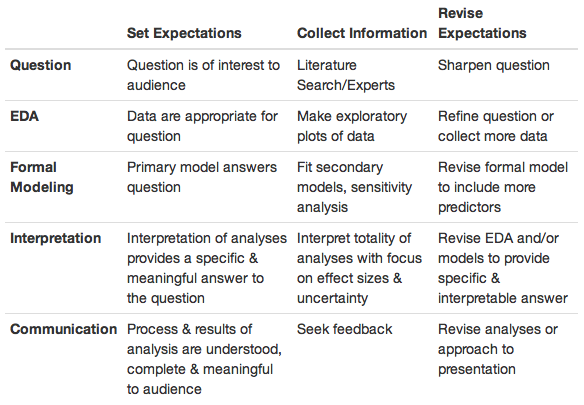
\includegraphics{03-img/1.png}
\caption{Figure 1}
\end{figure}

Although the process has divided into 5 step, these step are not statics
and usually this is not a linear from 1 to 5. There are a lot of
iterations until the last step.

\subsection{Step 1 - Ask a Question}\label{step-1---ask-a-question}

Usually all the analysis starts based on a question (good one), which we
would like to answer using data. Sometimes we already have these data
and we need to ``think'' what is a good question to this data (probabily
later you'll need more data). Generally, you do not have data but you
have a question and you'll need to find a good data set. This question
must have 5 features:

\begin{itemize}
\tightlist
\item
  Interest
\item
  Answerable
\item
  Specific
\item
  Pausible
\item
  Not already answered
\end{itemize}

Keep in mind that the question must be specific. If the question is not
specific, we must refine it.

\subsection{Step 2 - Wrangle}\label{step-2---wrangle}

This step is quite different from the Roger one, because here we deal
with:

\begin{itemize}
\tightlist
\item
  Gathering: If you do not have data you need to find it;

  \begin{itemize}
  \tightlist
  \item
    Download from the database stored in the webs;
  \item
    API
  \item
    Web Scraping
  \end{itemize}
\item
  Assess: Assess the quality of the data and the structure.

  \begin{itemize}
  \tightlist
  \item
    Structural problems: Different files with same information, but
    distincts column names
  \item
    Missing data
  \item
    incorrect data type
  \item
    duplicates
  \end{itemize}
\item
  Clean: Modifying the data to ensure the quality.
\end{itemize}

All this steps were to prepare the data to an analysis.

Sometimes Wrangling and EDA are binded into one step, but here are
splited.

\subsection{Step 3 - EDA}\label{step-3---eda}

Here we perform the EDA (Exploratory Data Analysis), discover some
patterns, relationships, descriptive analysis, maximize the potential of
the analysis, visualizations, and models. Also, removing outliers, and
creating new descriptive features from existind data.

\begin{itemize}
\tightlist
\item
  Exploring
\item
  Augment
\end{itemize}

In this step usually we need to revisit the question and refine with the
knowledge gathered (change the question or need more data).

\subsection{Step 4 - Draw Conclusions}\label{step-4---draw-conclusions}

This is step was to predict something (machine learning or inferencial
statistics).

\subsection{Step 5 - Communicate}\label{step-5---communicate}

Communicate the results.

\subsection{Packages}\label{packages}

In this course, three packages will be used massively.

\begin{itemize}
\tightlist
\item
  Numpy
\end{itemize}

\begin{Shaded}
\begin{Highlighting}[]
\ImportTok{import}\NormalTok{ numpy }\ImportTok{as}\NormalTok{ np}
\end{Highlighting}
\end{Shaded}

Convention: Abbreviate numpy as np.

\begin{itemize}
\tightlist
\item
  Pandas
\end{itemize}

\begin{Shaded}
\begin{Highlighting}[]
\ImportTok{import}\NormalTok{ pandas }\ImportTok{as}\NormalTok{ pd}
\end{Highlighting}
\end{Shaded}

Convention: Pandas numpy as pd.

\begin{itemize}
\tightlist
\item
  matplotlib
\end{itemize}

\begin{Shaded}
\begin{Highlighting}[]
\ImportTok{import}\NormalTok{ pandas }\ImportTok{as}\NormalTok{ pd}
\OperatorTok{%}\NormalTok{ matplotlib inline}
\end{Highlighting}
\end{Shaded}

\subsection{\texorpdfstring{\texttt{Methods}}{Methods}}\label{methods-3}

Methods used during the course videos.

\subsubsection{\texorpdfstring{\texttt{read\_csv()}}{read\_csv()}}\label{read_csv}

\begin{Shaded}
\begin{Highlighting}[]
\NormalTok{df }\OperatorTok{=}\NormalTok{ pd.read_csv(}\StringTok{'student_scores.csv'}\NormalTok{)}
\NormalTok{df }\OperatorTok{=}\NormalTok{ pd.read_csv(}\StringTok{'student_scores.csv'}\NormalTok{, sep}\OperatorTok{=}\StringTok{':'}\NormalTok{)}
\end{Highlighting}
\end{Shaded}

Import the dataframe.

\subsubsection{\texorpdfstring{\texttt{.head()}}{.head()}}\label{head}

\begin{Shaded}
\begin{Highlighting}[]
\NormalTok{df.head()}
\end{Highlighting}
\end{Shaded}

Show the first 5 rows

\subsubsection{\texorpdfstring{\texttt{.shape}}{.shape}}\label{shape}

\begin{Shaded}
\begin{Highlighting}[]
\NormalTok{df.shape()}
\end{Highlighting}
\end{Shaded}

Prints the dimenions.

\subsubsection{\texorpdfstring{\texttt{.dtypes}}{.dtypes}}\label{dtypes}

Prints the types of each variable.

\subsubsection{\texorpdfstring{\texttt{.info()}}{.info()}}\label{info}

Display a summary of each variable.

It is good to find missing values.

\subsubsection{\texorpdfstring{\texttt{.nunique()}}{.nunique()}}\label{nunique}

Return the number the unique values.

\subsubsection{\texorpdfstring{\texttt{.describe()}}{.describe()}}\label{describe}

This is a real summary.

\subsubsection{\texorpdfstring{\texttt{.tail()}}{.tail()}}\label{tail}

The last 5 rows.

\subsubsection{\texorpdfstring{\texttt{loc} and
\texttt{iloc}}{loc and iloc}}\label{loc-and-iloc}

Selecting the columns using \textbf{names}.

\begin{Shaded}
\begin{Highlighting}[]
\NormalTok{df_means }\OperatorTok{=}\NormalTok{ df.loc[:,}\StringTok{'id'}\NormalTok{:}\StringTok{'fractal_dimension_mean'}\NormalTok{]}
\end{Highlighting}
\end{Shaded}

Subsetting columns from ``id'' to ``fractal\_dimension\_mean''.

Same range of columns but using \textbf{index}.

\begin{Shaded}
\begin{Highlighting}[]
\CommentTok{# repeat the step above using index numbers}
\NormalTok{df_means }\OperatorTok{=}\NormalTok{ df.iloc[:,:}\DecValTok{11}\NormalTok{]}
\end{Highlighting}
\end{Shaded}

\subsubsection{\texorpdfstring{\texttt{.duplicated()}}{.duplicated()}}\label{duplicated}

Return a boolean vector., which could be useful to count the number of
duplicated.

\subsubsection{\texorpdfstring{\texttt{.drop\_duplicated()}}{.drop\_duplicated()}}\label{drop_duplicated}

Show the data set cleaned without duplicated, but do not update the
original dataframe to do it so you need to set inplace as True.

\begin{itemize}
\tightlist
\item
  inplace = True
\end{itemize}

\subsubsection{\texorpdfstring{\texttt{.mean()}}{.mean()}}\label{mean}

\begin{Shaded}
\begin{Highlighting}[]
\NormalTok{df[}\StringTok{"desired_column"}\NormalTok{].mean()}
\end{Highlighting}
\end{Shaded}

Mean function.

\subsubsection{\texorpdfstring{\texttt{.fillna(X)}}{.fillna(X)}}\label{fillnax}

Fill the NA with X.

\begin{itemize}
\tightlist
\item
  Alternativaly you can add inplace to update the current dataframe.
\end{itemize}

\subsubsection{\texorpdfstring{\texttt{pd.to\_daytime(df{[}\textquotesingle{}time\textquotesingle{}{]})}}{pd.to\_daytime(df{[}'time'{]})}}\label{pd.to_daytimedftime}

Update the object of time, but you need to assign to the dataframe
columns to change it.

\subsubsection{\texorpdfstring{\texttt{.hist()}}{.hist()}}\label{hist}

\begin{Shaded}
\begin{Highlighting}[]
\NormalTok{data.hist()}

\NormalTok{data.hist(figsize }\OperatorTok{=}\NormalTok{ (}\DecValTok{8}\NormalTok{,}\DecValTok{8}\NormalTok{)) }\CommentTok{# Biger figures.}

\NormalTok{data[}\StringTok{'age'}\NormalTok{].hist() }\CommentTok{# For a specific variable/featues.}
\end{Highlighting}
\end{Shaded}

Plot a simple histogram, beware because if you have many feactures, the
histogram going to be crowded.

\subsubsection{.plot()}\label{plot}

\begin{Shaded}
\begin{Highlighting}[]
\NormalTok{data[}\StringTok{'age'}\NormalTok{].plot(kind}\OperatorTok{=}\StringTok{'hist'}\NormalTok{)}\OperatorTok{;} \CommentTok{# Different way to plot a hist()}
\NormalTok{data[}\StringTok{'age'}\NormalTok{].plot(kind}\OperatorTok{=}\StringTok{'bar'}\NormalTok{)}\OperatorTok{;} \CommentTok{# Different way to plot a hist()}
\NormalTok{data[}\StringTok{'age'}\NormalTok{].plot(kind}\OperatorTok{=}\StringTok{'pie'}\NormalTok{,figsize}\OperatorTok{=}\NormalTok{ (}\DecValTok{8}\NormalTok{,}\DecValTok{8}\NormalTok{))}\OperatorTok{;} \CommentTok{# Different way to plot a hist()}

\CommentTok{# Matrix}
\NormalTok{pd.plotting.scatter_matrix(data,figsize}\OperatorTok{=}\NormalTok{(}\DecValTok{15}\NormalTok{,}\DecValTok{15}\NormalTok{))}

\CommentTok{# Scatter regular}
\NormalTok{data.plot(x }\OperatorTok{=} \StringTok{"compactness"}\NormalTok{, y }\OperatorTok{=} \StringTok{"concavity"}\NormalTok{ , kind }\OperatorTok{=} \StringTok{"scatter"}\NormalTok{)}

\CommentTok{# Boxplot}
\NormalTok{data[}\StringTok{'concave_points'}\NormalTok{].plot(kind }\OperatorTok{=} \StringTok{"box"}\NormalTok{)}
\end{Highlighting}
\end{Shaded}

\subsubsection{\texorpdfstring{\texttt{value\_counts()}}{value\_counts()}}\label{value_counts}

Aggregates counts for each new unique value in a column. Shows a vector
with this values.

\begin{Shaded}
\begin{Highlighting}[]
\NormalTok{data[}\StringTok{'something'}\NormalTok{].value_counts().plot(kind }\OperatorTok{=} \StringTok{'bar'}\NormalTok{)}\OperatorTok{;} \CommentTok{# Creates a bar ploat based on the value_counts created before.}
\end{Highlighting}
\end{Shaded}

\subsection{Subsetting}\label{subsetting}

\begin{Shaded}
\begin{Highlighting}[]
\NormalTok{data[data[}\StringTok{'anything'}\NormalTok{] }\OperatorTok{==} \StringTok{"M"}\NormalTok{] }\CommentTok{# data['anything'] == "M" -> will select each row with True.}
\end{Highlighting}
\end{Shaded}

\subsection{Indexing}\label{indexing}

\begin{Shaded}
\begin{Highlighting}[]
\CommentTok{# Example 1}
\NormalTok{ind }\OperatorTok{=}\NormalTok{ data[}\StringTok{'something'}\NormalTok{].value_counts().index}
\NormalTok{data[}\StringTok{'something'}\NormalTok{].value_counts()[index].plot(kind}\OperatorTok{=}\StringTok{'bar'}\NormalTok{) }\CommentTok{# Indexing!!}

\CommentTok{# Example 2}
\NormalTok{ind }\OperatorTok{=}\NormalTok{ data[}\StringTok{'anything'}\NormalTok{].value_counts().index}
\NormalTok{df[}\StringTok{'anything'}\NormalTok{].value_counts()[index].plot(kind}\OperatorTok{=}\StringTok{'pie'}\NormalTok{,figsize }\OperatorTok{=}\NormalTok{ (}\DecValTok{8}\NormalTok{,}\DecValTok{8}\NormalTok{))}
\end{Highlighting}
\end{Shaded}

\section{Data Analysis Process - Case Study
I}\label{data-analysis-process---case-study-i}

\section{Data Analysis Process - Case Study
II}\label{data-analysis-process---case-study-ii}

\section{Programming Workflow for Data
Analysis}\label{programming-workflow-for-data-analysis}

\section{Project Overview
(Instructions)}\label{project-overview-instructions-1}

\subsection{Overview}\label{overview-1}

In this project, you will analyze a dataset and then communicate your
findings about it. You will use the Python libraries NumPy, pandas, and
Matplotlib to make your analysis easier.

Preparation for this project with:
\href{https://classroom.udacity.com/courses/ud170-nd}{Intro to Data
Analysis}

\subsection{What do I need to install?}\label{what-do-i-need-to-install}

You will need an installation of Python, plus the following libraries:

\begin{verbatim}
* pandas
* NumPy
* Matplotlib
* csv
\end{verbatim}

We recommend installing Anaconda, which comes with all of the necessary
packages, as well as iPython notebook. You can find installation
instructions here.

\subsection{Why this Project?}\label{why-this-project}

In this project, you'll go through the data analysis process and see how
everything fits together. Later Nanodegree projects will focus on
individual pieces of the data analysis process.

You'll use the Python libraries NumPy, pandas, and Matplotlib, which
make writing data analysis code in Python a lot easier! Not only that,
these are sought-after skills by employers!

\subsection{What will I learn?}\label{what-will-i-learn}

After completing the project, you will:

\begin{itemize}
\tightlist
\item
  Know all the steps involved in a typical data analysis process
\item
  Be comfortable posing questions that can be answered with a given
  dataset and then answering those questions
\item
  Know how to investigate problems in a dataset and wrangle the data
  into a format you can use
\item
  Have practice communicating the results of your analysis
\item
  Be able to use vectorized operations in NumPy and pandas to speed up
  your data analysis code
\item
  Be familiar with pandas' Series and DataFrame objects, which let you
  access your data more conveniently
\item
  Know how to use Matplotlib to produce plots showing your findings
\end{itemize}

\subsection{2. Project Details}\label{project-details-1}

\subsubsection{How do I Complete this
Project?}\label{how-do-i-complete-this-project}

This project is connected with the Introduction to Data Analysis course,
but depending on your background knowledge, you may not need to take the
whole class to complete this project.

\subsubsection{Introduction}\label{introduction}

For the final project, you will conduct your own data analysis and
create a file to share that documents your findings. You should start by
taking a look at your dataset and brainstorming what questions you could
answer using it. Then you should use Pandas and NumPy to answer the
questions you are most interested in, and create a report sharing the
answers. You will not be required to use inferential statistics or
machine learning to complete this project, but you should make it clear
in your communications that your findings are tentative. This project is
open-ended in that we are not looking for one right answer.

\subsubsection{Step One - Choose Your Data
Set}\label{step-one---choose-your-data-set}

Click this link to open a document with links and information about data
sets that you can investigate for this project. You must choose one of
these datasets to complete the project.

\subsubsection{Step Two - Get Organized}\label{step-two---get-organized}

Eventually you'll want to submit your project (and share it with
friends, family, and employers). Get organized before you begin. We
recommend creating a single folder that will eventually contain:

\begin{itemize}
\tightlist
\item
  The report communicating your findings
\item
  Any Python code you wrote as part of your analysis
\item
  The data set you used (which you will not need to submit)
\end{itemize}

You may wish to use Jupyter notebook, in which case you can submit both
the code you wrote and the report of your findings in the same document.
Otherwise, you will need to submit your report and code separately. If
you would like a notebook template to help organize your investigation,
you can find a link in the resources at the bottom of the page or you
can click here. You can also complete and submit the project in the
classroom by going to the Project Notebook part of this lesson.

\subsubsection{Step Three - Analyze Your
Data}\label{step-three---analyze-your-data}

Brainstorm some questions you could answer using the data set you chose,
then start answering those questions. You can find some questions in the
data set options to help you get started.

Try and suggest questions that promote looking at relationships between
multiple variables. You should aim to analyze at least one dependent
variable and three independent variables in your investigation. Make
sure you use NumPy and Pandas where they are appropriate!

\subsubsection{Step Four - Share Your
Findings}\label{step-four---share-your-findings}

Once you have finished analyzing the data, create a report that shares
the findings you found most interesting. If you use a Jupyter notebook,
share your findings alongside the code you used to perform the analysis.
make sure that your report text is contained in Markdown cells to
clearly distinguish your comments and findings from your code work. You
should also feel free to use other tools and software to craft your
final report, but make sure that you can submit your report as an HTML
or PDF file so that it can be opened easily.

\subsubsection{Step Five - Review}\label{step-five---review}

Use the Project Rubric to review your project. If you are happy with
your submission, then you're ready to submit your project. If you see
room for improvement, keep working to improve your project!

\subsection{3. Video}\label{video}

\subsection{4. Investigate a Dataset}\label{investigate-a-dataset}

\subsection{Project Submission}\label{project-submission}

Choose one of Udacity's curated datasets and investigate it using NumPy
and pandas. Go through the entire data analysis process, starting by
posing a question and finishing by sharing your findings.

\subsection{Evaluation}\label{evaluation}

Use the Project Rubric to review your project. If you are happy with
your submission, then you are ready to submit! If you see room for
improvement in any category in which you do not meet specifications,
keep working!

Your project will be evaluated by a Udacity reviewer according to the
same Project Rubric. Your project must ``meet specifications'' or
``exceed specifications'' in each category in order for your submission
to pass.

\subsection{Submission}\label{submission}

\subsubsection{What to include in your
submission}\label{what-to-include-in-your-submission}

\begin{enumerate}
\def\labelenumi{\arabic{enumi}.}
\tightlist
\item
  A PDF or HTML file containing your analysis. This file should include:
\end{enumerate}

\begin{itemize}
\tightlist
\item
  A note specifying which dataset you analyzed
\item
  A statement of the question(s) you posed
\item
  A description of what you did to investigate those questions
\item
  Documentation of any data wrangling you did
\item
  Summary statistics and plots communicating your final results
\end{itemize}

\begin{enumerate}
\def\labelenumi{\arabic{enumi}.}
\setcounter{enumi}{1}
\tightlist
\item
  Code you used to perform your analysis. If you used a Jupyter
  notebook, you can submit your .ipynb. Otherwise, you should submit the
  code separately in .py file(s).
\item
  A list of Web sites, books, forums, blog posts, github repositories,
  etc. that you referred to or used in creating your submission (add N/A
  if you did not use any such resources).
\end{enumerate}

\subsubsection{Jupyter notebook
instructions}\label{jupyter-notebook-instructions}

If you used a Jupyter notebook on your computer to create your project,
you can include all your code and analysis in the notebook and do not
need to create additional files for your analysis. You will still need
to export your work in a PDF or HTML format also (see point 1 above),
and include this in your submission as well. To download your notebook
as an HTML file, click on File -\textgreater{} Download.As
-\textgreater{} HTML (.html) within the notebook. If you get an error
about ``No module name'', then open a terminal and try installing the
missing module using pip install (don't include the ``\textless{}'' or
``\textgreater{}'' or any words following a period in the module name).

\subsubsection{Ready to submit your
project?}\label{ready-to-submit-your-project}

Click on the ``Submit Project'' button and follow the instructions to
submit!

It can take us up to a week to grade the project, but in most cases it
is much faster. You will get an email when your submission has been
reviewed.

If you are having any problems submitting your project or wish to check
on the status of your submission, please email us at
\href{mailto:review-support@udacity.com}{\nolinkurl{review-support@udacity.com}}.

\bibliography{book.bib,packages.bib}


\end{document}
